\documentclass[12pt]{book}
\usepackage[letterpaper, margin=1in]{geometry}
\usepackage{graphicx}
\usepackage{wrapfig}
\usepackage{caption}
\usepackage{floatrow}
\usepackage{array}
\usepackage{tabularx}
\usepackage{hyperref}
\usepackage{tcolorbox}
\usepackage{longtable}
\usepackage{amsmath}

\graphicspath{{images/}}

\setlength\parindent{0pt}
\setlength\itemsep{0em}

\title{The Elder Scrolls Tabletop Roleplaying Game Player's Handbook}
\author{William Taylor Cook and Pascalle Audrey Nelson}

\begin{document}

\maketitle

\section*{Note from the Authors}
This game is a non-profit fan production intended to turn the complex and storied Elder Scrolls setting into a playable pencil-and-paper RPG. Elder Scrolls and all products under its name are owned by Bethesda Softworks and Bethesda Game Studios. We do not intend to profit off of this in any way. Please support the creators by buying their games and products.\\~\\
By participating in our game as a playtester, you agree to the following terms:

\begin{enumerate}
	\item You will not sell any portion of this game under any circumstances.
	\item You acknowledge that any rules and game mechanics may be subject to change by the authors in the service of better gameplay.
	\item You agree to help foster an inclusive, respectful atmosphere for all players. While we trust you all to do this, it bears repeating.
\end{enumerate}
In return, we promise the following to you:

\begin{enumerate}
	\item Our top priority is and always will be the creation of a satisfying gameplay experience.
	\item We will attempt to implement game changes in an unobtrusive way whenever possible.
	\item We will treat players with respect both out-of-character and in the way we create our narrative (even if player characters may not be respected).
	\item We encourage you to voice your concerns in any way you feel comfortable and will listen to your feedback.
\end{enumerate}
We hope you enjoy our game!
\newpage

\section*{About the Game}

Elder Scrolls is a vast, intricate fantasy setting. Attempting to compile relevant information here would be an effort in futility without a specific time and place in mind, and these rules are easily applicable to any setting throughout much of the Second, Third and early Fourth Eras. The game is largely based on the game mechanics of Elder Scrolls IV: Oblivion and Elder Scrolls III: Morrowind. Some modification would be necessary to make it function more like Elder Scrolls V and set it later in the Fourth Era, but it is possible if you were inclined to do so. For now, please refer to online sources for lore information. In particular, the Unofficial Elder Scrolls Project is a comprehensive and accurate source for information about all things Elder Scrolls. Much of the lore material here is taken from UESP --- a benefit of this being a not-for-profit fan creation.


\tableofcontents

\chapter{Basic Gameplay}
Before you begin making a character, you should understand the basic mechanics underlying the game. To play, you will need four-sided, six-sided, eight-sided, ten-sided, twelve-sided, twenty-sided and percentile dice. You can get away with only having one of each, but having multiple may make rolls easier. Dice are abbreviated according to how many sides they have. A d4 has four sides; a d10 has ten sides. Easy enough? This abbreviation can also accept a coefficient. If you are told to roll 2d6, that means to roll two six-sided dice and add their outcomes.

\section{Roleplaying}
The Elder Scrolls Tabletop Role Playing Game is a game focused on roleplaying. It's right in the name! Though you will find this book full of numbers, multipliers and percentages, all these formulas only exist to support a narrative. That narrative is the primary manner in which you will play this game.\\

Scenes in this game will typically follow a simple pattern. First, the GM will describe the scene and what is present in it. Next, the players describe how their characters act in relation to that scene. Then the GM narrates the outcome of that interaction. Whenever there is uncertainty about what the outcome of an action will be, the GM will ask the player to make an appropriate roll. The roll will decide what happens. Examples of such situations include attacks and skill-based actions.

\section{Making a Roll}
Whenever you are called upon to make a roll to determine success, you will need to roll a d10 and a percentile die. The percentile die determines the tens place, and the d10 determines the ones place. For example, if you roll a 40 on the percentile die and a 3 on the d10, your roll is 43. Some ten-sided dice are numbered 1-10 while others are numbered 0-9; rolling a 0 or a 10 counts as a 0 for the ones place. If you roll a 00 on the percentile die and a 0 on the d10, that means your roll is a 100.\\

Whatever the outcome of your roll, you will usually be asked to compare it to the value of a certain skill. Having a Blade skill of 40, for example, means you have a 40\% chance of succeeding whenever you roll to determine success on attacks with bladed weapons. This is accomplished by comparing the outcome of your roll to that value. To succeed on a roll, the outcome of that roll must be less than or equal to the specified value.

\subsection{Levels of Success}
Rolls are not all pass or fail. This game features \textit{success levels}, which are very important for opposed skill checks and may result in special bonuses! The outcomes of a roll are as follows:

\begin{figure}[h]
\begin{tabular}{p{0.3\textwidth}p{0.7\textwidth}}
	\textbf{Fumble} & 96-100\\
	\textbf{Failure} & Greater than your skill\\
	\textbf{Success} & Less than your skill\\
	\textbf{Hard Success} & Less than half your skill\\
	\textbf{Extreme Success} & Less than one-fifth of your skill\\
\end{tabular}
\end{figure}

\begin{tcolorbox}
	\textbf{Note}: If you are making a check using a skill that is 50 or higher, only rolls 98 or higher count as a fumble.
\end{tcolorbox}

Fumbling on a roll is a critical failure. You will lose an opposed roll even if your opponent fails, and you may face abnormally bad consequences at the GM's discretion, such as being disarmed or knocked off your feet in battle. Regular failures will typically mean you simply do not accomplish your goal, on the other hand. Extreme successes will sometimes grant even more than you asked for. Achieving extreme success on an attack will do maximum damage, for instance (see \textit{Chapter 4, Combat}).\\

If a task seems like it is harder than usual, the GM may require you to make a hard or even extreme success to accomplish it. Some rules specify the conditions under which this occurs. For example, if you make a ranged attack that is greater than the range of your weapon (but less than double), it requires a hard success to hit!

\subsection{Opposed Rolls}
Whenever two characters are acting in opposition of each other, they must both make rolls to see which one performs better. Success levels are very important here; the character who achieves the higher success level wins. Ties result in no clear victor unless a tiebreaking condition is specified. For example, ties on opposed attack/defense rolls generally go to the defender (see \textit{Chapter 4, Combat}).

\subsection{Bonus and Penalty Dice}
Whenever a roll has a bonus die, reroll the percentile die and take the lower result. Remember that lower is better. Penalty dice have the opposite effect: the higher roll takes effect instead of the lower one.\\

\begin{tcolorbox}
\textbf{Example 1}: Thoronir Greenhollow wants to climb a tree to get a better view of the area. The GM decides this requires a normal Acrobatics check, meaning Thoronir must roll at or below his Acrobatics score. His Acrobatics score is 50, giving him a reasonable chance of succeeding. However, he is exhausted, giving him a penalty die on the roll. He rolls a 40 on his percentile die and a 5 on his d10, meaning his roll is a success! However, the reroll of the percentile die comes up with a 60, changing his roll to 65, meaning he failed.\\

\textbf{Example 2}: Rasha-daro is trying to sneak by a guard. The GM asks her player to make a Sneak check. It is night, and Rasha-daro's path across the room is only dimly lit. This gives her a bonus die. She needs to roll below her Sneak score of 40 to succeed. She rolls a 45, failing; however, she gets to reroll the percentile die, changing her roll to 15. She winds up with a hard success on the roll!
\end{tcolorbox}

\subsubsection{Multiple Bonuses and Penalties}
When there are multiple bonus or penalty conditions affecting a roll, they have a cumulative effect. There can be multiple dice added to the roll. For example, if you have two bonus dice on your roll, you take the best of three percentile die rolls. Wherever a roll has bonus \textit{and} penalty dice, the two cancel each other out. For example, a roll with three penalty dice and two bonus dice will wind up with only one penalty die.

\section{Non-Integer Values}
Wherever non-integer values are the final result of a calculation, always round down. For example, if your Destruction spells cost 99\% of their base cost, a spell with a base cost of 6 magicka will now have a cost of 5 magicka, even though $6*0.99=5.94$. However, intermediate values you use while completing a formula are not rounded.

\chapter{Character Creation}
Creating a character in the Elder Scrolls Tabletop RPG is a multi-step process with many options for customization. You can choose from 10 races, each with different attributes and traits. You also choose the astrological sign under which your character was born, granting further bonuses. On top of that, there are also 21 skills and 21 classes --- you can even make your own custom class! The choices can seem overwhelming, so let's take this one step at a time.

\section{Stats}

As you create your character, you will assign numbers that represent your character's physical and mental abilities. These numbers are called \textit{attributes,} and they come in two kinds: primary and derived. Primary attributes have an indirect effect on your character, and they are largely determined by your race and birthsign. They are as follows:

\begin{figure}[h]
\begin{tabular}[h]{p{0.15\textwidth}p{0.85\textwidth}}
	\textbf{Strength} & Muscle power. Determines your melee damage bonus.\\
	\textbf{Intelligence} & Mental acuity. Determines your maximum magicka.\\
	\textbf{Willpower} & Strength of will. Determines your magicka regeneration rate and spell range.\\
	\textbf{Agility} & Coordination. Determines your ranged weapon damage bonus.\\
	\textbf{Speed} & Rate of bodily movement. Determines your per-round movement speed.\\
	\textbf{Endurance} & Physical health and toughness. Determines your maximum health.\\
	\textbf{Personality} & Charm and beauty. Sets NPCs' initial opinions of you.\\
\end{tabular}
\end{figure}

Your derived attributes have a more direct impact on your character.
\begin{figure}[h]
\begin{tabular}[h]{p{0.4\textwidth}p{0.6\textwidth}}
	\textbf{Health} & General condition of your body.\\
	\textbf{Magicka} & Stored magical energy.\\
	\textbf{Stamina} & Ability to endure physical exertion.\\
	\textbf{Magicka Regeneration Rate} & How quickly your magicka recovers.\\
	\textbf{Stamina Regeneration Rate} & How quickly your stamina recovers.\\
	\textbf{Movement} & Your per-round rate of movement.\\
	\textbf{Damage Bonus} & The damage you add to attacks.\\
\end{tabular}
\end{figure}

The Luck attribute from Oblivion is not used, for simplicity. Now that you understand attributes, it is time to start building your character.

\section{Races}
There are ten playable races which represent the ten mainstream cultures of Tamriel. Each comes with a starting set of attributes as well as skill bonuses and special traits or powers. Each race is listed here along with a picture, description, and stats. Don't write this all in pen - it'll be changing!\\

Races begin the game with the stats listed in the following table:
\begin{figure}[h]
\begin{tabular}[h]{|p{0.1\textwidth}|p{0.1\textwidth}p{0.1\textwidth}p{0.1\textwidth}p{0.1\textwidth}p{0.1\textwidth}p{0.1\textwidth}p{0.1\textwidth}|}
	\hline
	\textbf{Race} & STR & INT & WIL & AGI & SPD & END & PER\\
	\hline
	Altmer & 30 & 50 & 40 & 40 & 35 & 35 & 40\\
	\hline
	Argonian & 40 & 45 & 35 & 45 & 45 & 30 & 30\\
	\hline
	Bosmer & 30 & 40 & 30 & 50 & 50 & 35 & 35\\
	\hline
	Breton & 35 & 50 & 50 & 30 & 35 & 30 & 40\\
	\hline
	Dunmer & 40 & 40 & 30 & 40 & 50 & 35 & 35\\
	\hline
	Imperial & 40 & 40 & 35 & 30 & 35 & 40 & 50\\
	\hline
	Khajit & 35 & 40 & 30 & 50 & 40 & 35 & 40\\
	\hline
	Nord & 50 & 30 & 35 & 40 & 40 & 45 & 30\\
	\hline
	Orc & 45 & 35 & 45 & 35 & 30 & 50 & 30\\
	\hline
	Redguard & 45 & 30 & 30 & 40 & 40 & 50 & 35\\
	\hline
\end{tabular}
\end{figure}

\subsection{Altmer (High Elf)}
\begin{wrapfigure}{L}{0.3\textwidth}
	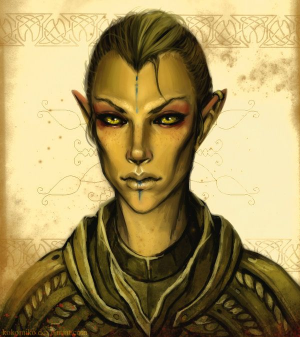
\includegraphics[width=\textwidth]{Altmer.png}
\end{wrapfigure}

The Altmer, or self-titled ``Cultured People', are a tall, golden-skinned race, hailing from Summerset Isle. They are also known as High Elves by the denizens of Tamriel. In the Empire, ``High'' is often understood to mean proud or snobbish, and as the Altmer generally personify these characteristics, the ``lesser races'' generally resent them. Altmer live two to three times as long as humans; with a 200-year-old Altmer being old and a 300-year-old Altmer being very, very old. Altmer consider themselves to be the most civilized culture of Tamriel; the common tongue of the continent is based on Altmer speech and writing, and most of the Empire's arts, crafts, laws, and sciences are derived from Altmer traditions. They usually have golden, green, or amber eyes.\\

The Altmer are the most strongly gifted in the arcane arts of all the races, and they are very resistant to diseases. However, they are also somewhat vulnerable to magicka, fire, frost, and shock, which makes them very weak against their strongest point --- magic. They are among the longest living and most intelligent races of Tamriel, and they often become powerful magic users due to both their magical affinity and the many years they may devote to their studies.\\

Altmer get the following skill bonuses: +5 Alchemy, +10 Alteration, +5 Conjuration, +10 Destruction, +5 Illusion, +10 Mysticism.\\

Altmer have a permanent +100 bonus to max magicka and a 75\% resistance to disease; however, they have a 25\% vulnerability to fire, frost and shock damage.

\subsection{Argonian}
\begin{wrapfigure}{L}{0.3\textwidth}
	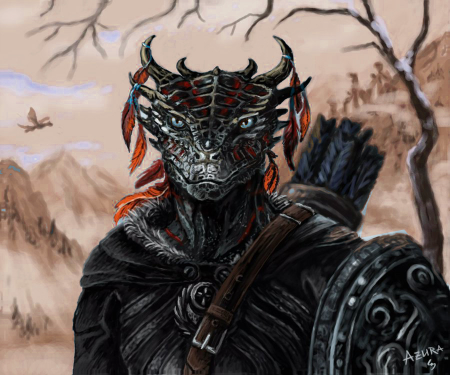
\includegraphics[width=\textwidth]{Argonian.png}
\end{wrapfigure}

Argonians (in their native tongue of Jel they call themselves the Saxhleel, or People of the Root) are the reptilian natives of Black Marsh, a vast swampland province in southeastern Tamriel. The other races often prefer to refer to them as 'lizards' or the 'Lizard Folk' instead, especially when meaning to be derogative. They are known as the foremost experts in guerrilla warfare throughout the Starry Heart, a reputation brought upon them by defending their borders from enemies for countless centuries. Argonians have a lifespan similar to that of humans. According to the First Era Scholar Brendan the Persistent "the Argonian people have, throughout Tamrielic history, been perhaps the most misunderstood, vilified, and reviled of all the sentient races. Yet, those who have taken the time to experience Argonian culture have gained a greater appreciation for this noble and beautiful people." However, it should be noted that he himself went missing in his final expedition into the deeper swamps of their homeland.\\

Argonians get the following skill bonuses: +5 Alchemy, +10 Athletics, +5 Blade, +5 Hand-to-Hand, +5 Illusion, +5 Mysticism, +10 Security.\\

They have a complete immunity to poison and a 75\% resistance to disease. They can breathe underwater and are adept swimmers, suffering no movement penalty or melee attack penalty in water.

\subsection{Bosmer (Wood Elf)}
\begin{wrapfigure}{L}{0.3\textwidth}
	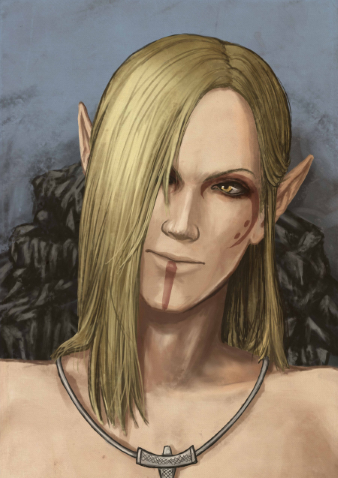
\includegraphics[width=\textwidth]{Bosmer.png}
\end{wrapfigure}

The Bosmer are the Elven clan-folk of Valenwood, a forested province in southwestern Tamriel. In the Empire, they are often referred to as Wood Elves, but Bosmer, Boiche, or the Tree-Sap people is what they call themselves. Bosmer rejected the stiff, formal traditions of Aldmeri high culture, preferring a more romantic, simple existence in harmony with the land and its wild beauty and creatures. They are relatively nimble and quick in body compared to their more "civilized" Altmeri cousins (who often look down upon the Bosmer as unruly and naive). Their agility makes them well-suited as scouts and thieves. However, they are also a quick-witted folk, and many pursue successful careers in scholarly pursuits or trading. Bosmer live two to three times as long as humans; with a 200-year-old Bosmer being old and a 300-year-old Bosmer being very, very old. Though they are considered less influential than some of their Elven brethren, the Bosmer are also relatively prone to producing offspring. As a result, they outnumber all other mer on Tamriel.\\

The best archers in all of Tamriel, the Bosmer snatch and fire arrows in one continuous motion; they are even rumored to have invented the bow. They have many natural and unique abilities; notably, they can command simple-minded creatures and have a nearly chameleon-like ability to hide in forested areas. Many in the forests of Valenwood follow the tenets of the Green Pact. These "Green Pact Bosmer" are religiously carnivorous and cannibalistic, and do not harm the vegetation of Valenwood, though they are not averse to using wooden or plant-derived products created by others.\\

Bosmer get the following skill bonuses: +5 Acrobatics, +10 Alchemy, +5 Alteration, +5 Light Armor, +10 Marksman, +10 Sneak.\\

Bosmer have a 75\% resistance to disease. They get the Beast Tongue power as well, which lets them control lesser animals for 1 minute once a day.

\subsection{Breton}
\begin{wrapfigure}{L}{0.3\textwidth}
	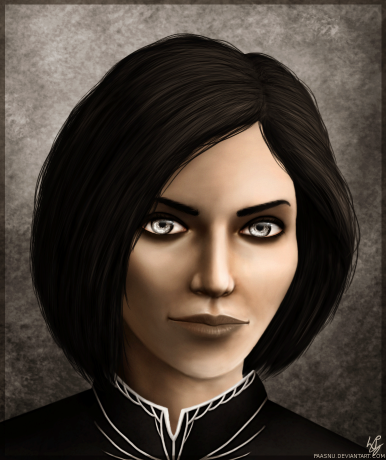
\includegraphics[width=\textwidth]{Breton.png}
\end{wrapfigure}

Bretons are the human descendants of the Aldmeri-Nedic Manmer of the Merethic Era and are now the inhabitants of the province of High Rock. They are united in culture and language, even though they are divided politically, for High Rock is a fractious region. Bretons make up the peasantry, soldiery, and magical elite of the feudal kingdoms that compete for power. Many are capable mages with innate resistance to magicka. They are known for a proficiency in abstract thinking and unique customs. Bretons appear, by and large, much like other pale-skinned humans. They are usually slight of build and not as muscular as Nords or Redguards. Their Elvish ancestry is usually only detectable upon a closer inspection of their eyebrows, ears, or high cheekbones, though many individual Bretons appear to be more Nordic or Imperial than anything else. The great diversity in their appearance is to be expected from their politically fractured society, though their clothes, accents, customs and names are fairly uniform.\\

Bretons get the following skill bonuses: +5 Alchemy, +5 Alteration, +10 Conjuration, +5 Illusion, +10 Mysticism, +10 Restoration.\\

They have a natural 50\% resistance to magic and gain a permanent +50 bonus to max magicka. Their Dragon Skin power gives them 50\% physical resistance for 1 minute, once a day.

\subsection{Dunmer (Dark Elf)}
\begin{wrapfigure}{L}{0.3\textwidth}
	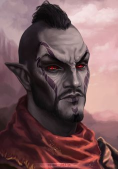
\includegraphics[width=\textwidth]{Dunmer.png}
\end{wrapfigure}

The Dunmer, also known as Dark Elves, are the ash-skinned, typically red-eyed elven peoples of Morrowind. ``Dark'' is commonly understood as meaning such characteristics as ``dark-skinned'', ``gloomy'', ``ill-favored by fate'' and so on. The Dunmer and their national identity, however, embrace these various connotations with enthusiasm. In the Empire, ``Dark Elf'' is the common usage, but among their Aldmeri brethren they are called ``Dunmer''. Their combination of powerful intellects with strong and agile physiques produce superior warriors and sorcerers. On the battlefield, Dunmer are noted for their skill with a balanced integration of the sword, the bow and destruction magic. Dunmer live two to three times as long as humans; with a 200-year-old Dunmer being old and a 300-year-old Dunmer being very, very old. In character, they are grim, aloof, and reserved, as well as distrusting and disdainful of other races.\\

Dunmer distrust and are treated distrustfully by other races. They are often proud, clannish, ruthless, and cruel, from an outsider's point of view, but greatly value loyalty and family. Young female Dunmer have a reputation for promiscuity in some circles. Despite their powerful skills and strengths, the Dunmer's vengeful nature, age-old conflicts, betrayals, and ill-reputation prevent them from gaining more influence. Those born in their homeland of Morrowind are known to be considerably less friendly than those who grew up in the Imperial tradition.\\

Dunmer get the following skill bonuses: +5 Athletics, +10 Blade, +5 Blunt, +10 Destruction, +5 Light Armor, +5 Marksman, +5 Mysticism.\\

Dunmer have a natural 75\% resistance to fire. They can also summon an ancestral spirit to aid them in battle for 1 minute, once a day.

\newpage % Gets the float to align properly
\subsection{Imperial}
\begin{wrapfigure}{l}{0.3\textwidth}
	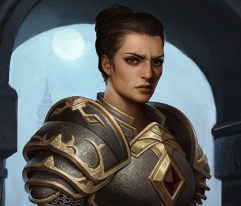
\includegraphics[width=\textwidth]{Imperial.png}
\end{wrapfigure}

Also known as Cyrodiils, Cyrodilics, Cyro-Nordics and Imperial Cyrods, the well-educated and well-spoken Imperials are the natives of the civilized, cosmopolitan province of Cyrodiil. Imperials are also known for the discipline and training of their citizen armies, and their respect for the rule of law. Though physically less imposing than the other races, the Imperials have proved to be shrewd diplomats and traders, and these traits, along with their remarkable skill and training as light infantry, have enabled them to subdue all the other nations and races and erect the monument to peace and prosperity that comprises the Glorious Empire. Their hegemony has waxed and waned throughout the eras, and most historians refer to three distinct Empires, the ends of which each mark a new epoch in Tamrielic history.\\

Imperials get the following skill bonuses: +5 Blade, +5 Blunt, +5 Hand-to-Hand, +10 Heavy Armor, +10 Mercantile, +10 Speechcraft.\\

Imperials gain two major powers: Star of the West, which lets them absorb 100 stamina on touch once per day, and Voice of the Emperor, which charms a target for 30 seconds once per day.

\subsection{Khajiit}
\begin{wrapfigure}{l}{0.3\textwidth}
	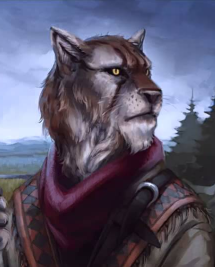
\includegraphics[width=\textwidth]{Khajiit.png}
\end{wrapfigure}

Khajiit are cat-like people who come from Elsweyr, known for high intelligence and agility. These traits make them very good thieves and acrobats, but Khajiit are also fearsome warriors. However, they are rarely known to be mages. Khajiit mostly stay on land, but piracy and skooma trade does draw some to work as sailors.\\

Khajiit anatomy differs greatly from both men and elves, not only because of their fur, tail, and sometimes toe-walking stance, but also their digestive system and metabolism. Khajiit, Argonians, and Imga are the so-called ``beast races'' of Tamriel because of these large differences. Khajiit have a lifespan similar to that of humans. There are no well-documented cases of cross-breeding between Khajiit and other races, though there are rumors of such a thing. The foreign appearance and behavior of Khajiit make them common targets of racial discrimination.\\

Khajiit get the following skill bonuses: +10 Acrobatics, +5 Athletics, +5 Blade, +10 Hand-to-Hand, +5 Light Armor, +5 Security, +5 Sneak.\\

Khajiit have cat eyes that allow them to see in the dark and claws that boost their unarmed attack damage to 1d6+DB. In addition to this, the Eye of Fear power lets them inflict fear for 3 rounds on a single target who can see them, once a day.

\subsection{Nord}
\begin{wrapfigure}{l}{0.3\textwidth}
	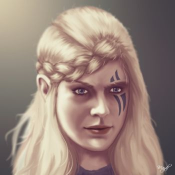
\includegraphics[width=\textwidth]{Nord.png}
\end{wrapfigure}

The Nords are the children of the sky, a race of tall and fair-haired humans from Skyrim who are known for their incredible resistance to cold and magical frost. They are fierce, strong and enthusiastic warriors, and many become renowned warriors, soldiers and mercenaries all over Tamriel. Eager to augment their martial skills beyond the traditional methods of Skyrim, they excel in all manner of warfare, and are known as a militant people by their neighbors. Nords are also natural seamen, and have benefited from nautical trade since their first migrations from Atmora. They captain and crew many merchant fleets, and may be found all along the coasts of Tamriel.\\

Nords get the following skill bonuses: +5 Armorer, +10 Blade, +5 Block, +10 Blunt, +10 Heavy Armor, +5 Restoration.\\

Nords have a 50\% resistance to frost damage and can channel Nordic Frost to deal 50 points of frost damage on touch once per day. The Woad power grants them 30\% physical damage reduction for one minute once per day.

\subsection{Orc}
\begin{wrapfigure}{l}{0.3\textwidth}
	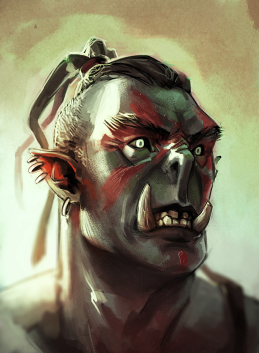
\includegraphics[width=\textwidth]{Orc.png}
\end{wrapfigure}

Orcs, also called Orsimer or "Pariah Folk" in ancient times, are sophisticated, beastlike people of the Wrothgarian Mountains, Dragontail Mountains, Valenwood, and Orsinium (literally translated as ``Orc-Town''). They are noted for their unshakable courage in war and their unflinching endurance of hardships. Orcs have elven blood, but are usually considered to be beastfolk. In the past, Orcs have been widely feared and hated by the other nations and races of Tamriel, and were often considered to be goblin-ken. However, they have slowly won acceptance in the Empire, in particular for their distinguished service in the Emperor's Legions. Orc armorers are prized for their craftsmanship, and Orc warriors in heavy armor are among the finest front-line troops in the Empire, and are fearsome when using their berserker rage. Orcs have a lifespan similar to that of humans. Most Imperial citizens regard the Orc society as rough and cruel. The Orcs of the Iliac Bay region have developed their own language, known as Orcish, and have often had their own kingdom, Orsinium.\\

Orcs get the following skill bonuses: +10 Armorer, +5 Block, +10 Blunt, +5 Hand-to-Hand, +10 Heavy Armor.\\

Orcs have a natural 25\% resistance to magic. Once a day they may enter a berserk state for 1 minute, which grants the following effects: Fortify Stamina 200, Fortify Health 20, Fortify Strength 50, Drain Agility 100.

\subsection{Redguard}
\begin{wrapfigure}{l}{0.3\textwidth}
	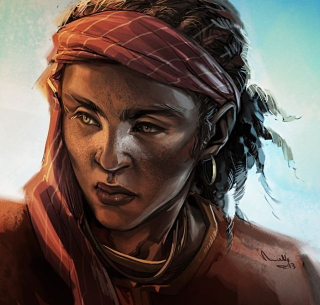
\includegraphics[width=\textwidth]{Redguard.png}
\end{wrapfigure}

Redguards are the most naturally talented warriors in Tamriel. The dark-skinned, wiry-haired people of Hammerfell seem born to battle, though their pride and fierce independence of spirit makes them more suitable as scouts or skirmishers, or as free-ranging heroes and adventurers, than as rank-and-file soldiers. In addition to their cultural affinities for many armor styles and weapons (particularly swords), Redguards are also physically blessed with hardy constitutions, resistance to poison, and quickness of foot. Redguards do not share the same blood as the other human races, and they have no known connection with the ancestral Nordic homeland of Atmora.\\

Redguards get the following skill bonuses: +10 Athletics, +10 Blade, +10 Blunt, +5 Heavy Armor, +5 Light Armor, +5 Mercantile.\\

Hardy of constitution, Redguards have a natural 75\% resistance to poison and disease. Once a day, they can have an Adrenaline Rush which grants the following effects for 1 minute: Fortify Agility 50, Fortify Endurance 50, Fortify Speed 50, Fortify Strength 50, Fortify Health 25.\\

\begin{tcolorbox}
Be sure to take note of all your race's skill bonuses and abilities. Skills will be covered in greater detail in the next chapter, so you may wish to come back here once you learn more about them.
\end{tcolorbox}

\section{Birthsigns}
The people of Tamriel mark their calendars by the passage of constellations overhead. When the sun passes near one, it is that constellation's season. There are thirteen in total: one for each month of the year and then one which seems to wander intermittently, giving it no predictable season. This collection of constellations is known as the Firmament, and many attribute personality traits to the sign under which one was born. The signs of the Firmament are listed here in chronological order; each one grants a certain bonus which may include attribute increases and powers.

\begin{longtable}{lm{0.6\textwidth}}
	\raisebox{-0.5\height}{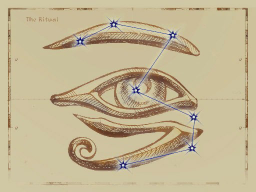
\includegraphics[width=0.3\textwidth]{Ritual.png}} & \textbf{The Ritual}: The month of Morning Star is marked by the Ritual, a sign denoting a deep connection with the moons and the Divines. Those born under the ritual gain two powers: Mara's Gift (allows them to heal themselves for 200 their health once a day) and Blessed Word (causes undead to flee for 3 rounds for 40 magicka).\\
	
	\raisebox{-0.5\height}{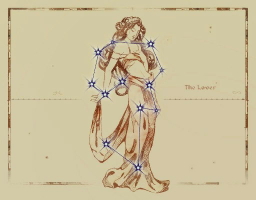
\includegraphics[width=0.3\textwidth]{Lover.png}} & \textbf{The Lover}: Those born in the month of Sun's Dawn under the Lover are said to be passionate and graceful. The Lover bestows the Lover's Kiss power, which allows the user to paralyze a target on touch for one round at the cost of 120 stamina damage.\\

	\raisebox{-0.5\height}{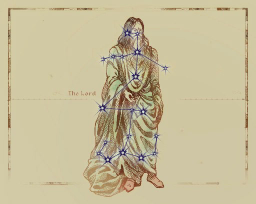
\includegraphics[width=0.3\textwidth]{Lord.png}} & \textbf{The Lord}: The Lord marks the month of First Seed, where he oversees all the planting in Tamriel. Those born under the Lord are said to be healthier than usual and are granted the Blood of the North power, allowing them to heal 45 health per round for 2 rounds at the cost of 50 magicka. However, they are also cursed with Troll's Blood, giving them a 25\% weakness to fire.\\

	\raisebox{-0.5\height}{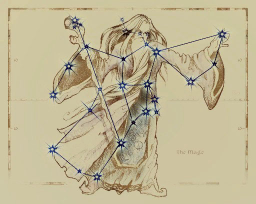
\includegraphics[width=0.3\textwidth]{Mage.png}} & \textbf{The Mage}: One of the three guardian signs, the Mage marks the month of Rain's Hand, when magicka was first used by humans. Those born under the Mage are particularly gifted in the arcane arts and gain a permanent +50 bonus to maximum magicka.\\

	\raisebox{-0.5\height}{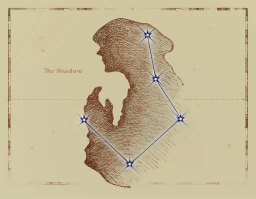
\includegraphics[width=0.3\textwidth]{Shadow.png}} & \textbf{The Shadow}: The Shadow's season is the month of Second Seed. This sign grants those born under it the power of Moonshadow, which lets them turn invisible for one minute, once a day.\\

	\raisebox{-0.5\height}{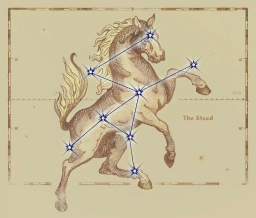
\includegraphics[width=0.3\textwidth]{Steed.png}} &
\textbf{The Steed}: Those born in the month of Mid Year under the sign of the Steed are impatient, always hurrying from place to place and restless whenever they have to wait. They gain a permanent +20 bonus to their Speed attribute.\\

\raisebox{-0.5\height}{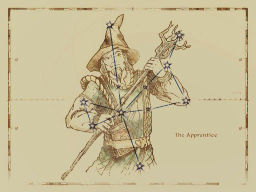
\includegraphics[width=0.3\textwidth]{Apprentice.png}} & \textbf{The Apprentice}: The month of Sun's Height is the season of the Apprentice. Those born under this sign are especially gifted with magic and gain a permanent +100 to max magicka; however, they also gain a permanent 100\% vulnerability to magic.\\

\raisebox{-0.5\height}{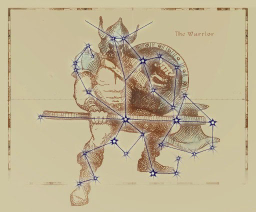
\includegraphics[width=0.3\textwidth]{Warrior.png}} & \textbf{The Warrior}: The Warrior is another of the guardian signs. It marks the month of Last Seed and is said to grant those born in this month skill with weapons of all kinds as well as a short temper. This sign grants a permanent +10 bonus to both Endurance and Strength.\\

\raisebox{-0.5\height}{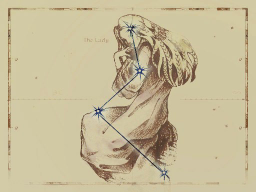
\includegraphics[width=0.3\textwidth]{Lady.png}} & \textbf{The Lady}: The Lady presides graciously over the month of Heartfire. Those born under this sign are said to be kind and tolerant, and they gain a permanent +10 bonus to both Willpower and Endurance.\\

\raisebox{-0.5\height}{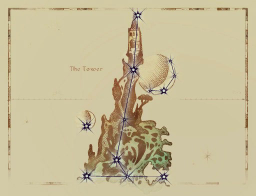
\includegraphics[width=0.3\textwidth]{Tower.png}} & \textbf{The Tower}: The Tower is a birthsign of great fortune, and those born under it are said to find treasure in one way or another. The Tower grants two powers: Tower Key (open a lock of average level or lower for free once a day) and Tower Warden (5\% chance to reflect incoming damage back to the target for 1 minute).\\

\raisebox{-0.5\height}{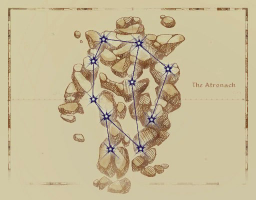
\includegraphics[width=0.3\textwidth]{Atronach.png}} & \textbf{The Atronach}: A sign representing elemental beings from Oblivion, the Atronach is both a blessing and a curse to aspiring mages. Those born under the Atronach gain a permanent +150 bonus to maximum magicka and have a 50\% chance to absorb spells targeting them (meaning they have no effect and you gain the magicka used to cast the spell). However, they cannot regenerate magicka on their own.\\

\raisebox{-0.5\height}{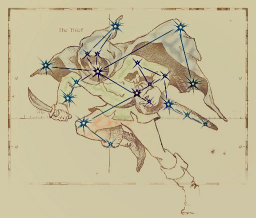
\includegraphics[width=0.3\textwidth]{Thief.png}} & \textbf{The Thief}: The final month of the year is Evening Star, and it is marked by the guardian sign of the Thief. Those born under the Thief are not necessarily thieves; instead, they are prone to risky lifestyles and rarely come to harm due to their natural luck. They receive a permanent +10 bonus to both Speed and Agility.\\

\raisebox{-0.5\height}{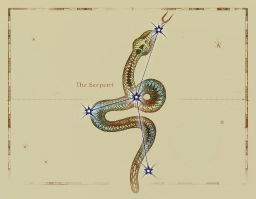
\includegraphics[width=0.3\textwidth]{Serpent.png}} & \textbf{The Serpent}: There are no common characteristics amongst those born under the Serpent, but they are said to be the most blessed and the most cursed. The Serpent grants the power of Serpent Spell, which has the following effects: the user may touch a target and damage them for 30 health per round for 2 rounds; whether or not a target is touched, the user is cured of poison, all magical effects of Expert level or lower are dispelled, and 100 stamina points are lost. This power may be used once per day.\\
\end{longtable}

\section{Classes}
There are a grand total of 21 classes in the Elder Scrolls Tabletop RPG, each with a unique combination of favored skills and attributes. You may wish to become more acquainted with what the skills mean in order to make an informed decision about which class you choose.\\

A class consists of 4 components:
\begin{enumerate}
	\item A name.
	\item A specialization (combat, magic or stealth).
	\item Two favored primary attributes.
	\item Seven major skills.
\end{enumerate}

All skills grouped under the chosen specialization get a +5 bonus. The two favored attributes gain a +5 bonus as well. The seven major skills gain a +20 bonus; the remaining 14 skills are defined as minor skills. If you wish to create a custom class, simply choose the four components on your own. You should look over the 21 existing classes, however -- odds are you'll find multiple appealing choices.\\

\begin{longtable}{lm{0.6\textwidth}}
	\raisebox{-0.5\height}{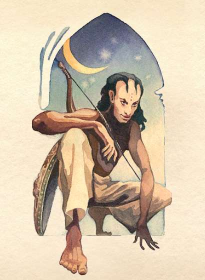
\includegraphics[width=0.3\textwidth]{Acrobat.png}} & 
\textbf{\Large Acrobat}\newline

The kind of person that uses agility and endurance to their advantage. Unafraid of jumping long distances.\newline

\textbf{Specialization}: Stealth\newline
\textbf{Attributes}: Agility, Endurance\newline
\textbf{Skills}: Acrobatics, Blade, Block, Marksman, Security, Sneak, Speechcraft\\

	\raisebox{-0.5\height}{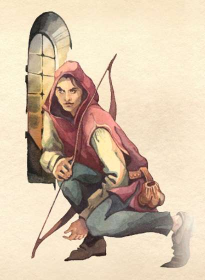
\includegraphics[width=0.3\textwidth]{Agent.png}} & \textbf{\Large Agent}\newline

Charming when they can be seen, and nearly invisible when in shadow.\newline

\textbf{Specialization}: Stealth\newline
\textbf{Attributes}: Agility, Personality\newline
\textbf{Skills}: Acrobatics, Illusion, Marksman, Mercantile, Security, Sneak, Speechcraft\\

	\raisebox{-0.5\height}{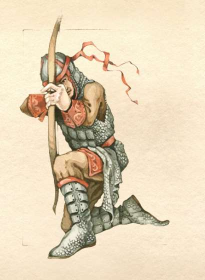
\includegraphics[width=0.3\textwidth]{Archer.png}} & \textbf{\Large Archer}\newline

A marksman, adept at combat at great distances. Able to take down most foes before they have a chance to draw sword.\newline

\textbf{Specialization}: Combat\newline
\textbf{Attributes}: Agility, Strength\newline
\textbf{Skills}: Armorer, Blade, Blunt, Hand-to-Hand, Light Armor, Marksman, Sneak\\

	\raisebox{-0.5\height}{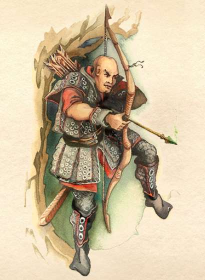
\includegraphics[width=0.3\textwidth]{Assassin.png}} & \textbf{\Large Assassin}\newline

Nimble and quiet, they move in darkness to strike at the unsuspecting. Locks hold no doors shut for them.\newline

\textbf{Specialization}: Stealth\newline
\textbf{Attributes}: Intelligence, Speed\newline
\textbf{Skills}: Acrobatics, Alchemy, Blade, Light Armor, Marksman, Security, Sneak\\

	\raisebox{-0.5\height}{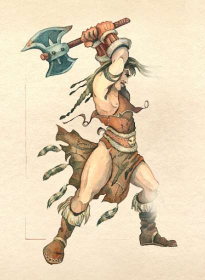
\includegraphics[width=0.3\textwidth]{Barbarian.png}} & \textbf{\Large Barbarian}\newline

Fearsome brutes who inspire fear and dread in the hearts of their enemies. Like a storm, swift and powerful. Finding little use for heavy armor, they rely on smashing their foes into the ground.\newline

\textbf{Specialization}: Combat\newline
\textbf{Attributes}: Speed, Strength\newline
\textbf{Skills}: Armorer, Athletics, Blade, Block, Blunt, Hand-to-Hand, Light Armor\\

	\raisebox{-0.5\height}{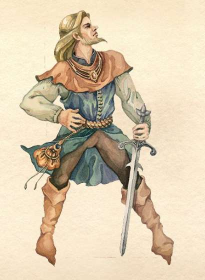
\includegraphics[width=0.3\textwidth]{Bard.png}} & \textbf{\Large Bard}\newline

Intelligent and personable, they prefer to accomplish tasks with their words first, and sword second.\newline

\textbf{Specialization}: Stealth\newline
\textbf{Attributes}: Intelligence, Personality\newline
\textbf{Skills}: Alchemy, Blade, Block, Illusion, Light Armor, Mercantile, Speechcraft\\

	\raisebox{-0.5\height}{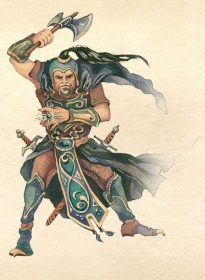
\includegraphics[width=0.3\textwidth]{Battlemage.png}} & \textbf{\Large Battlemage}\newline

Able to resolve most conflicts with either spell or sword. They are a deadly mix of scholar and soldier.\newline

\textbf{Specialization}: Magic\newline
\textbf{Attributes}: Intelligence, Strength\newline
\textbf{Skills}: Alchemy, Alteration, Blade, Blunt, Conjuration, Destruction, Mysticism\\

	\raisebox{-0.5\height}{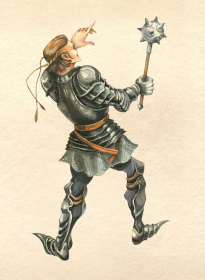
\includegraphics[width=0.3\textwidth]{Crusader.png}} & \textbf{\Large Crusader}\newline

A combatant who wields the power of brute strength and medicinal knowledge. Cheating death after every fight, they rely on their keen knowledge of restoration to fight yet again.\newline

\textbf{Specialization}: Combat\newline
\textbf{Attributes}: Strength, Willpower\newline
\textbf{Skills}: Athletics, Blade, Blunt, Destruction, Hand-to-Hand, Heavy Armor, Restoration\\

	\raisebox{-0.5\height}{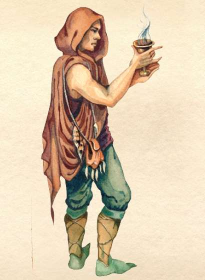
\includegraphics[width=0.3\textwidth]{Healer.png}} & \textbf{\Large Healer}\newline

Fighters of poison and illness. The ancient art of restoration is their ally, and the deadly art of destruction is their weapon.\newline

\textbf{Specialization}: Magic\newline
\textbf{Attributes}: Personality, Willpower\newline
\textbf{Skills}: Alchemy, Alteration, Destruction, Illusion, Mercantile, Restoration, Speechcraft\\

\raisebox{-0.5\height}{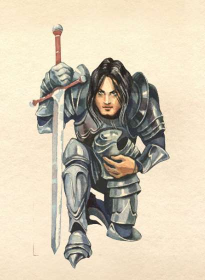
\includegraphics[width=0.3\textwidth]{Knight.png}} & \textbf{\Large Knight}\newline

The most noble of all combatants. Strong in body and in character.\newline

\textbf{Specialization}: Combat\newline
\textbf{Attributes}: Personality, Strength\newline
\textbf{Skills}: Blade, Block, Blunt, Hand-to-Hand, Heavy Armor, Illusion, Speechcraft\\

	\raisebox{-0.5\height}{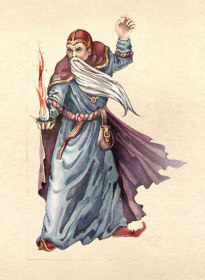
\includegraphics[width=0.3\textwidth]{Mageclass.png}} & \textbf{\Large Mage}\newline

Preferring to use their extensive knowledge of all things magical, they wield a might more powerful than the sharpest blade.\newline

\textbf{Specialization}: Magic\newline
\textbf{Attributes}: Intelligence, Willpower\newline
\textbf{Skills}: Alchemy, Alteration, Conjuration, Destruction, Illusion, Mysticism, Restoration\\

\raisebox{-0.5\height}{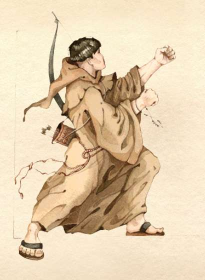
\includegraphics[width=0.3\textwidth]{Monk.png}} & \textbf{\Large Monk}\newline

Quick and cunning with the empty hand, they are strong in spirit. They prefer to solve conflict by arrow or by fist.\newline

\textbf{Specialization}: Stealth\newline
\textbf{Attributes}: Agility, Willpower\newline
\textbf{Skills}: Acrobatics, Alteration, Athletics, Hand-to-Hand, Marksman, Security, Sneak\\

\raisebox{-0.5\height}{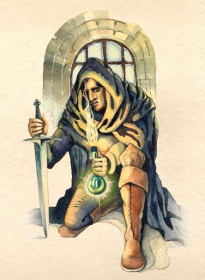
\includegraphics[width=0.3\textwidth]{Nightblade.png}} & \textbf{\Large Nightblade}\newline

Spell and shadow are their friends. By darkness they move with haste, casting magic to benefit their circumstances.\newline

\textbf{Specialization}: Magic\newline
\textbf{Attributes}: Speed, Willpower\newline
\textbf{Skills}: Acrobatics, Alteration, Athletics, Blade, Destruction, Light Armor, Restoration\\

\raisebox{-0.5\height}{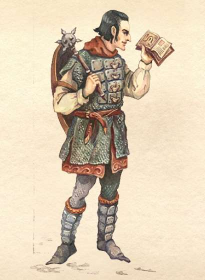
\includegraphics[width=0.3\textwidth]{Pilgrim.png}} & \textbf{\Large Pilgrim}\newline

Hearty folk, well-versed in the tomes of old. They profit in life by bartering in the market, or by persuading the weak-minded.\newline

\textbf{Specialization}: Stealth\newline
\textbf{Attributes}: Endurance, Personality\newline
\textbf{Skills}: Armorer, Block, Blunt, Light Armor, Mercantile, Security, Speechcraft\\

	\raisebox{-0.5\height}{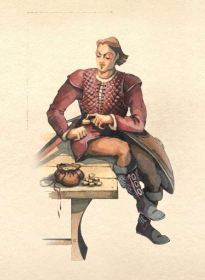
\includegraphics[width=0.3\textwidth]{Rogue.png}} &
\textbf{\Large Rogue}\newline

They use speed in combat rather than brute force. Persuasive in conversation, their tongues are as sharp as blades.\newline

\textbf{Specialization}: Combat\newline
\textbf{Attributes}: Personality, Speed\newline
\textbf{Skills}: Alchemy, Athletics, Blade, Block, Illusion, Light Armor, Mercantile\\


	\raisebox{-0.5\height}{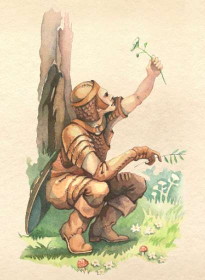
\includegraphics[width=0.3\textwidth]{Scout.png}} &
\textbf{\Large Scout}\newline

Preferring the rolling countryside to the city life, they are gifted with the ability to evade, guard and protect themselves with great proficiency.\newline

\textbf{Specialization}: Combat\newline
\textbf{Attributes}: Endurance, Speed\newline
\textbf{Skills}: Acrobatics, Alchemy, Armorer, Athletics, Blade, Block, Light Armor\\

	\raisebox{-0.5\height}{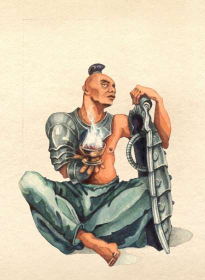
\includegraphics[width=0.3\textwidth]{Sorcerer.png}} & \textbf{\Large Sorcerer}\newline

Besting the most well-equipped fighters, they rely on the spells of the mystic arts. Unique to these mages is the bodily stamina to be armed with the thickest armor.\newline

\textbf{Specialization}: Magic\newline
\textbf{Attributes}: Endurance, Intelligence\newline
\textbf{Skills}: Alchemy, Alteration, Conjuration, Destruction, Heavy Armor, Mysticism, Restoration\\

	\raisebox{-0.5\height}{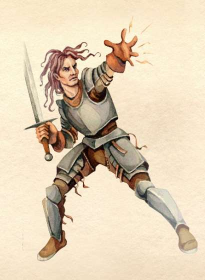
\includegraphics[width=0.3\textwidth]{Spellsword.png}} & \textbf{\Large Spellsword}\newline

More nimble and athletic than the sorcerer, and better suited for spell-casting than the knight, their attacks are unpredictable. Students of combat and magic.\newline

\textbf{Specialization}: Magic\newline
\textbf{Attributes}: Endurance, Willpower\newline
\textbf{Skills}: Alteration, Blade, Block, Heavy Armor, Destruction, Illusion, Restoration\\

	\raisebox{-0.5\height}{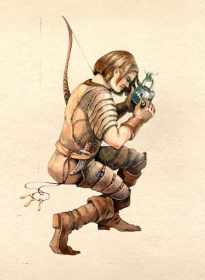
\includegraphics[width=0.3\textwidth]{Thiefclass.png}} & \textbf{\Large Thief}\newline

Profiting from the losses of others is their love. Able to be swift in shadow, and crafty in bartering. Locks are enemies, and lock-picks are their swords.\newline

\textbf{Specialization}: Stealth\newline
\textbf{Attributes}: Agility, Speed\newline
\textbf{Skills}: Acrobatics, Light Armor, Marksman, Mercantile, Security, Sneak, Speechcraft\\

	\raisebox{-0.5\height}{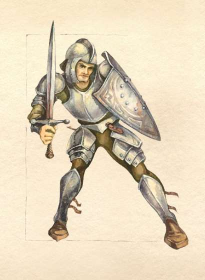
\includegraphics[width=0.3\textwidth]{Warriorclass.png}} & \textbf{\Large Warrior}\newline

Unafraid of light weaponry, they plow into the fray with little regard for injury. Masters of all melee tools, they put little faith in the magical arts.\newline

\textbf{Specialization}: Combat\newline
\textbf{Attributes}: Endurance, Strength\newline
\textbf{Skills}: Armorer, Athletics, Blade, Block, Blunt, Hand-to-Hand, Heavy Armor\\

	\raisebox{-0.5\height}{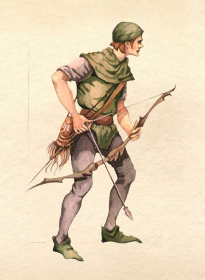
\includegraphics[width=0.3\textwidth]{Witchhunter.png}} & \textbf{\Large Witchhunter}\newline

Swift on foot, and clever with spells, they use distance as their ally. Slower adversaries are fodder for their arrows.\newline

\textbf{Specialization}: Magic\newline
\textbf{Attributes}: Agility, Intelligence\newline
\textbf{Skills}: Alchemy, Athletics, Conjuration, Destruction, Marksman, Mysticism, Security\\
\end{longtable}

\section{Derived Attributes}
Now is the time to calculate your derived attributes. There are a lot of things to keep track of here. Be sure to write them down so you don't have to do equations in your head all the time throughout gameplay.
\begin{itemize}
	\item $\text{Health}=2*\text{Endurance}$.
	\item $\text{Magicka}=2*\text{Intelligence}$.
	\item $\text{Stamina}=\text{Strength}+\text{Willpower}+\text{Agility}+\text{Endurance}$.
	\item You recover $(5+0.1*\text{Willpower})\%$ of your magicka per round.
	\item Your carry weight is equal to five times your Strength.
	\item Your spell range is equal to double your Willpower in feet. 
\end{itemize}

Your movement and damage bonuses are given by the following table.
\begin{center}
\begin{tabular}{|l|l|c|c|c|c|c|}
\hline
Derived Attribute & Attribute & 1--24 & 25--49 & 50--74 & 74--99 & 100\\ \hline
Damage Bonus (Melee) & Strength & +0 & +1 & +2 & +3 & +4 \\ \hline
Damage Bonus (Ranged) & Agility & +0 & +1 & +2 & +3 & +4 \\ \hline
Movement & Speed & 20 ft & 30 ft & 40 ft & 50 ft & 60 ft\\ \hline
\end{tabular}
\end{center}

\section{Skill Points}
By now, you should have all the information you need to finalize your skill points. The base value of any given skill is 5, so be sure to add all relevant bonuses to that. For example, a Breton Mage begins with a Conjuration of 5(base)+10(racial)+5(magic class)+20(major skill)=40. To learn more about what exactly the skills do, move on to chapter 3. In any case, your character is now complete! Congratulations!

\chapter{Skills}

There are 21 skills in the Elder Scrolls Tabletop RPG. Each one comes with a specialization (combat, magic or stealth), a governing attribute (contributes to attribute increases when you level up), and a set of mastery perks you get automatically when you reach certain skill levels.

In addition to providing mastery perks, skill levels determine your proficiency with using the skill. Certain actions will require you to make a skill check. In order to do so, simply roll percentile and compare it to your skill value. If it is less than or equal to your skill, it is a success. If it is less than or equal to half your skill value, it is a hard success. If it is less than or equal to one-fifth of your skill value, it is an extreme success. If it is greater than your skill value, it is a failure.

Some checks may have a higher difficulty level and require a hard or extreme success to pass them. Some checks are contests, and the character with the higher success level wins. If you roll a 96 or higher, your roll is considered a "fumble," which is a lower success level than a failure. The GM has the option to impose a penalty for fumbles. If you are at least a Journeyman of that skill, you can only fumble on a 98 or higher.

Some skills may also provide some bonuses such as spell cost reduction based on skill level. Thus, it's worth boosting stats even if you don't get the next mastery perk. These bonuses will be covered in their respective chapters. In this chapter, you'll find a list of all the skills along with their specializations, governing attributes, meanings and mastery perks.

\section{Skill List}

\begin{tabular}{p{0.2\textwidth}|p{0.2\textwidth}|p{0.15\textwidth}|p{0.45\textwidth}}

Skill & Specialization & Attribute & Uses\\ \hline
Acrobatics & Stealth & Speed & Jumping, climbing and dodging.\\ \hline
Alchemy & Magic & Intelligence & Crafting potions and poisons.\\ \hline
Alteration & Magic & Willpower & Casting spells to change physical properties.\\ \hline
Armorer & Combat & Endurance & Repairing and crafting equipment.\\ \hline
Athletics & Combat & Speed & Sprinting, swimming and stamina recovery.\\ \hline
Blade & Combat & Strength & Attacking with bladed weapons.\\ \hline
Block & Combat & Endurance & Blocking attacks with weapons and shields.\\ \hline
Blunt & Combat & Strength & Attacking with blunt weapons.\\ \hline
Conjuration & Magic & Intelligence & Conjuring minions and equipment from Oblivion.\\ \hline
Destruction & Magic & Willpower & Casting spells to harm foes directly.\\ \hline
Hand-to-Hand & Combat & Strength & Attacking with fists.\\ \hline
Heavy Armor & Combat & Endurance & Effectively using heavy armor.\\ \hline
Illusion & Magic & Personality & Magically manipulating sense and emotion.\\ \hline
Light Armor & Stealth & Speed & Effectively using light armor.\\ \hline
Marksman & Stealth & Agility & Attacking with ranged weapons.\\ \hline
Mercantile & Stealth & Personality & Haggling.\\ \hline
Mysticism & Magic & Intelligence & Casting Mysticism spells.\\ \hline
Restoration & Magic & Willpower & Fortifying stats and healing.\\ \hline
Security & Stealth & Agility & Bypassing locks and other security.\\ \hline
Sneak & Stealth & Agility & Moving silently and striking unseen.\\ \hline
Speechcraft & Stealth & Personality & Speaking persuasively.\\
\end{tabular}

\newpage
\section{Mastery Perks}

Skill levels are grouped into five tiers: Novice (0-24), Apprentice (25-49), Journeyman (50-74), Expert (75-99) and Master (100). Upon achieving each tier, you gain access to a special mastery perk. The following table lists each skill's mastery perks.

\begin{tabular}{p{0.15\textwidth}|p{0.12\textwidth}|p{0.15\textwidth}|p{0.15\textwidth}|p{0.13\textwidth}|p{0.15\textwidth}}

Skill & Novice & Apprentice & Journeyman & Expert & Master\\ \hline
Acrobatics & You can attempt to dodge melee attacks for 10 stamina. & Dodging no longer costs stamina. & Non-dodge acrobatics checks in combat cost 30 feet of movement instead of an action. & Non-dodge acrobatics checks in combat cost 15 feet of movement. & Your first dodge made between turns does not impose a penalty die on the next one.\\ \hline
Alchemy & You know the first effect of alchemical reagents. & You know the first two effects of alchemical reagents. & You know the first three effects of alchemical reagents. & You know all effects of alchemical reagents. & You can create potions from single ingredients.\\ \hline
Alteration & Can cast Novice Alteration spells. & Alteration spells last 1.5x as long & Protection spells are twice as effective on unarmored targets. & Absorb half magicka from offensive spells. & +25\% magic resistance.\\ \hline
Armorer & You can craft and repair weapons and armor. & Repair kits get twice as many uses. & You can repair magic items. & Repair kits get three times as many uses. & Repair kits may be used indefinitely.\\

\end{tabular}

\begin{tabular}{p{0.15\textwidth}|p{0.12\textwidth}|p{0.15\textwidth}|p{0.15\textwidth}|p{0.13\textwidth}|p{0.15\textwidth}}

Skill & Novice & Apprentice & Journeyman & Expert & Master\\ \hline
Athletics & Can sprint for double movement (30 stamina, action). & You have a swim movement of 20 feet. & Stamina recovers 40 points per round. & Stamina recovers 50 points per round. & Stamina recovers 60 points per round.\\ \hline
Blade & Blade technique: Power Attack & Blade technique: Standing Strike & Blade Technique: Flanking Strike & Blade Technique: Sweeping Attack & Blade Technique: Dizzying Blow\\ \hline
Block & You can attempt to block melee attacks for 10 stamina. & Blocking no longer costs stamina. & On an extreme success, the attacker suffers recoil. & On a success, 5\% chance of disarming attacker. & Your first block between turns does not impose a penalty die on your next reaction.\\ \hline
Blunt & Blunt technique: Power Attack & Blunt technique: Standing Strike & Blunt Technique: Flanking Strike & Blunt Technique: Sweeping Attack & Blunt Technique: Dizzying Blow\\ \hline
Conjuration & Novice Conjuration spells. & Conjuration spells last 1.5x as long. & Bound weapons banish daedra and turn undead at or below your level. & Minions gain +100 max health. & Can have two minions at once.\\

\end{tabular}

\begin{tabular}{p{0.15\textwidth}|p{0.12\textwidth}|p{0.15\textwidth}|p{0.15\textwidth}|p{0.13\textwidth}|p{0.15\textwidth}}

Skill & Novice & Apprentice & Journeyman & Expert & Master\\ \hline
Destruction & Novice Destruction spells. & Destruction Dual Casting. & On an extreme success, destruction spells stagger foes. & Elemental Mastery: Fire, Frost or Lightning. & Once a day, you may ignore 50\% resistance with a spell.\\ \hline
Hand-to-Hand & Unarmed technique: Power Attack & Unarmed technique: Standing Strike & Unarmed technique: Disarming Attack & Unarmed technique: Paralyzing Palm & Unarmed technique: Power Within\\ \hline
Hand-to-Hand (cont'd) & ... & ... & Unarmed attacks gain the Magical property; blocking recoils attackers on an extreme success. & Blocking grants a counterattack on an extreme success. & Disarm on extreme success for counterattack.\\ \hline
Heavy Armor & You can wear heavy armor. & Heavy armor no longer imposes penalty on Marksman rolls. & Heavy armor movement penalty is reduced by 5 ft. & Heavy armor movement penalty is reduced by 10 ft. & Heavy armor no longer imposes a movement penalty.\\ \hline
Illusion & Novice illusions. & Illusions last 1.5x as long. & Spellcasting is now silent. & Charms automatically increase NPC disposition. & Illusions affect undead, daedra and automatons.\\

\end{tabular}

\begin{tabular}{p{0.15\textwidth}|p{0.12\textwidth}|p{0.15\textwidth}|p{0.15\textwidth}|p{0.13\textwidth}|p{0.15\textwidth}}

Skill & Novice & Apprentice & Journeyman & Expert & Master\\ \hline
Light Armor & You can wear light armor. & Light armor movement penalty is reduced by 5 ft. & Light armor no longer imposes movement penalty. & Light armor weighs nothing when worn. & Stamina regenerates 50\% faster while you wear light armor.\\ \hline
Marksman & Archery technique: Aim & Archery technique: Volley; also aiming is free. & Archery technique: Trick Shot & Archery technique: Focus Shot & Archery technique: Snipe\\ \hline
Mercantile & You can buy and sell goods. & You can invest 500 gold into a shop; the vendor is now a fence. & You can sell any type of item to any vendor. & Invested shops permanently have an additional 500 gold. & All shops have an additional 500 gold available for bartering (stacks with expert).\\ \hline
Mysticism & Novice Mysticism spells. & Mysticism spells last 1.5x as long. & When your ward negates a spell, gain half of the magicka used to cast that spell. & Magic detection gives you precise information on item enchantments. & Magic detection allows you to detect all magical effects.\\ \hline
Restoration & Novice Restoration spells. & Restoration spells last 1.5x as long. & Healing spells are 0.5\% more powerful per skill level. & 1.25x multiplier on your magicka regeneration formula. & Healing spells restore stamina equal to half of health recovered.\\

\end{tabular}

\begin{tabular}{p{0.15\textwidth}|p{0.12\textwidth}|p{0.15\textwidth}|p{0.15\textwidth}|p{0.13\textwidth}|p{0.15\textwidth}}

Skill & Novice & Apprentice & Journeyman & Expert & Master\\ \hline
Security & Can automatically pick Very Easy locks. & Can automatically pick Easy locks. & Can automatically pick Average locks. & Can automatically pick Hard locks. & Can automatically pick Very Hard locks.\\ \hline
Sneak & Sneak attack damage: 2x ranged, 3x one-handed & Sneak attack damage: 3x ranged, 6x one-handed. & Dagger sneak attacks deal 15x damage. & You may move your full movement while sneaking. & Sneak attacks ignore armor.\\ \hline
Speechcraft & Can bribe NPCs to increase disposition. & Can attempt 4 Speechcraft checks in the same conversation. & Disposition losses from failures are halved. & Bribes cost half as much. & Once per day, guarantee an extreme success on a single check.\\

\end{tabular}

For more information about what combat techniques and spell perks mean, check out chapters 5 and 6.

\chapter{Combat}

The ESTRPG features a round-based combat system not unlike that of \textit{Dungeons \& Dragons}. The rules for combat and movement will seem very familiar to anyone who has played it before. However, some rules are different, so be sure to pay attention! This chapter describes the rules needed for characters to engage in combat.

\begin{figure}[H]
	\includegraphics[width=\textwidth]{combat.png}
\end{figure}

\section{The Order of Combat}

A round is defined as 6 seconds, and each combatant gets \textit{movement} and an \textit{action} on their turn. Turn order is decided by the Speed attribute. If two Speed attributes are the same, turn order is then decided among the tied combatants by their Agility attributes. If both of those are a tie, the GM decides turn order among NPCs and the players decide turn order among PCs. If there is a tie with both attributes among both NPCs and PCs, then flip a coin.

\subsection{Surprise}

Sometimes, you (or your enemy!) may have the chance to attack a target who is unaware. If a combatant is surprised, they do not get to react to the attack or take a turn until the next round. Surprise is determined by success on a Sneak check, which can be modified by several conditions. The following is gives examples, but is not exhaustive:

\begin{tabular}{p{0.3\textwidth}|p{0.3\textwidth}}

Bonus & Penalty\\ \hline
	\begin{itemize}
		\item In concealment or cover
		\item Disguised
		\item Beneficial spells
	\end{itemize}
	&
	\begin{itemize}
		\item Target suspects you
		\item Wearing heavy armor
		\item Target has locating spell
		\item Moving in difficult terrain
	\end{itemize}\\

\end{tabular}

Note that not all conditions may stack. Use your judgement for what makes narrative sense.

\subsection{Your Turn}
On your turn, you may move a distance no more than your maximum movement (as described in the next section) and take an \textit{action}. An action allows you to do certain things such as make an attack, cast a spell (see \textit{Chapter 6}) or execute a combat technique (see \textit{Chapter 5}). You will also regenerate a certain amount of stamina and magicka if they are not already at max, at a rate described in section 2.5. Some abilities do not require an action to execute. Abilities labeled as "reaction" may be executed in response to certain occurrences, such as being able to roll for Block when targeted in melee. Certain small actions like drawing or sheathing a weapon can be done in tandem with your movement and action.

\subsubsection{Bonus Actions}
Some actions may be listed as "bonus actions." This means that you may take this action for free on your turn; however, you only get one bonus action per round.

\subsection{Other Actions}
In addition to attacks and the abilities listed in chapters 5 and 6, the following count as an action that you may perform on your turn:

\begin{itemize}
	\item Disengage: Your movement this turn cannot provoke opportunity attacks (see \textit{section 5.2.1}).
	\item Evade: You focus exclusively on avoiding harm. Attacks against you (including ranged attacks) gain a penalty die. Does not stack with fast movement penalty dice.
	\item Help: You attempt to aid an ally. If they perform a non-combat check before their next turn, they gain a bonus die. If they make an attack against a creature within 5 feet of you, it gets a bonus die.
	\item Hide: You attempt to escape the notice of enemies. Make a Sneak check. On a success, you manage to slip away, at least for the moment. This does not mean enemies have absolutely no idea where you are, however; you cannot hide from a creature that can see you, and if you make noise, you give away your position.
	\item Prepare: You declare an action to be executed when a certain event occurs before your next turn.
	\item Sprint (\textit{20 Stamina}): You can forego your action to gain double your movement bonus. While you are sprinting, ranged attacks against you gain a penalty die. Argonians and apprentices of Athletics can take this action while swimming.
\end{itemize}

\section{Making an Attack}

To make an attack, simply spend your action for the round and declare a target. The target must be within range (5 ft for melee weapons, 10 ft for Reach melee weapons; ranged attacks have specific rules as described in chapter 5) and not be behind total cover. Ranged weapons use the skill check rules described in section 5.2.2. Melee attacks automatically succeed unless the target chooses to react by blocking or dodging. (It is assumed even a novice can hit a stationary target.) If they do, make a skill check with your relevant weapon skill and compare it to the target's success level on their Block or Acrobatics check. If your success level is higher, you have successfully hit the target and may roll your damage. Ties are decided according to which reaction the target chose to take: blocks and dodges win on a tie, but fighting back loses on a tie.

Please note: attacks with spells can be either melee or ranged attacks. Touch spells require an attack roll that obeys all the rules of melee combat, and ranged spells require an attack roll that obeys all the rules of ranged combat. Whatever bonus or penalty conditions might affect such rolls will also affect spell attacks.

\section{Movement in Combat}

Movement is the total distance you can move in a round without exerting yourself. It is determined by your Speed attribute, as described in section 2.5. On your turn, you can move up to that distance. Your movement may be split before and after your action if you wish, and you do not have to use your full movement. For example, you may move 10 feet, attack, then move 10 more feet if your movement is at least 20 feet. You get different max movements for different types of movement (e.g. walking and swimming). The distance you move by any means is subtracted from each movement type simultaneously. For example, if your walking movement is 30 ft and your swimming movement is 15, and you walk 10 feet then begin to swim, you can only swim an additional 5 feet that turn.

\subsection{Hazards and Penalties}
Some conditions may change your movement. Armor reduces your movement speed by a certain amount particular to the armor. Being prone requires an extra foot of movement for every foot you crawl (e.g. crawling 10 feet costs 20 feet of movement). Standing up from the prone position costs half of your current max movement. For example, if your movement is normally 30 feet and your armor imposes -10 to your movement, then your current max movement is 20 feet. Standing up would thus cost 10 feet of movement.

Some terrain types also slow movement because they are hazardous to traverse, such as a frozen river, rubble, a floor littered with broken glass, low furniture, steep stairs, deep snow, shallow swampland or undergrowth. These terrain types cost an additional foot of movement for every foot moved, and this effect stacks with crawling.

While sneaking, you can only move half your max movement.

\section{Mounted Combat}

Sometimes, you may engage in combat while riding a mount. In this case, you control the mount's turn and use its movement speed instead of yours. Its place in the turn order is the same as yours, calculated by your Speed. You may mount or dismount for half of your movement. If an effect moves your mount against your will while you are riding it, you must make an Athletics or Acrobatics check (your choice) to avoid falling off. If you fail, you land on the ground within 5 feet, prone. You must make the same check if you are targeted by effects that knock you prone. Mounts may only use their action to Evade or Sprint, though they can react with Dodge.

\section{Underwater Combat}

Fighting underwater comes with unique challenges that can seriously inhibit anyone not experienced in it or otherwise adapted to aquatic environents. Any combatants without a defined swim speed have a penalty die on all melee attacks with blunt weapons. Ranged weapon attacks automatically miss beyond base range and gain a penalty die otherwise. Spell attack range is halved. Creatures fully submersed in water gain 50\% resistance to fire damage. Unless you have water breathing, you can only hold your breath underwater for a number of minutes equal to one plus 5\% of your Endurance. After this time limit, you have a number of rounds equal to 5\% of your Endurance to reach the surface before your health drops to 0.

\section{Death and Healing}

\begin{wrapfigure}{l}{0.6\textwidth}
	\includegraphics[width=\textwidth]{victory.png}
\end{wrapfigure}

If your health drops to 0, you lose consciousness and are now dying. Gaining any amount of health will stabilize you and allow you to wake up. Restoration spells and healing potions will do so, but they must be administered by someone who is not incapacitated. Some items will allow you to stabilize a dying character but not heal them.

Dying characters who have not been stabilized are now in the hands of fate. Each turn, roll percentile. On a 50 or lower, mark a success. On a 51 or higher, mark a failure. A total of three successes means you are stable. A total of three failures means you are permanently dead. If you roll a 96 or higher, mark two failures; a roll of 5 or lower immediately grants 1 hit point.

If an attack reduces your health to 0 and there is damage remaining, you immediately die if the remainder is greater than or equal to half your max health. For example, if you have 30 of 60 health left and an attack does 60 damage, it reduces you to 0 health, and the remaining 30 damage equals your half your max health, killing you instantly.

If your stamina goes into the negative, you pass out, but are not dying. You regain stamina at a rate of 60 per round until your stamina is positive again and you regain consciousness. Be careful not to overexert yourself!

\chapter{Equipment \& Combat Techniques}

Weapons and armor offer a variety of combat options to those skilled in their use. Each weapon and weapon type has certain properties that affect the manner in which it is used and the effects it has on targets. Players are encouraged to explore different choices of armament to see which tactics are effective in which situations. You may find that certain weapon types are more effective against certain enemies; it is therefore advantageous to train multiple combat skills and use the right weapons for the job.

In addition to these basic properties, equipment also grants access to combat techniques --- special moves you can do that deal extra damage and have bonus effects. Most techniques become available as your skill with weapons increases, as described in the skill mastery perk table (\textit{section 3.2}). Some techniques are available to everyone and may be used regardless of which weapons one is wielding. However, combat techniques cost stamina, so be sure to pace yourself!

\section{Glossary of Weapon Properties}
\begin{itemize}
	\item Blade: This is a bladed weapon, and it uses the Blade skill for attack rolls. All bladed weapons are Impaling.
	\item Blunt: This is a blunt weapon, and it uses the Blunt skill for attack rolls. Blunt weapons ignore some armor points.
	\item Heavy: This weapon is so large and/or heavy that it cannot be used more than once per round under any conditions.
	\item Impaling: This weapon has a sharp edge or point; on an extreme success, weapons with this property deal max damage and then another base damage die. (e.g. a longsword (1d10+DB) deals 10 damage in addition to the normal damage bonus and another d10 roll.)
	\item Light: This weapon is small and light enough that it can be used up to three times in a round. It is also excellent for dual wielding.
	\item One-Handed: This weapon only requires one hand to use.
	\item Magic: This weapon has magical properties which may make it interact with certain enemies in unusual ways.
	\item Marksman: This is a bow, and it uses the Marksman skill. All bows are Impaling.
	\item Medium: This weapon's weight is between that of a light and a heavy weapon, and it can be used twice per round.
	\item Reach: This weapon's length extends your reach by 5 ft.
	\item Two-Handed: This weapon requires the use of two hands and therefore prevents dual wielding, the use of shields, and possibly other tasks requiring hands (at the GM's discretion).
\end{itemize}

In addition to these properties, specific weapons also have a Quality, which can grant extra damage compared to poorer weapons of the same type. They have a base damage die as well, listed before the properties. Remember to add your skill and attribute damage bonuses as well. You get +1 to all melee attacks for every 25 points of Strength and +1 to all ranged attacks for every 25 points of Agility. Skills work the same way: every 25 points in a skill gives you a permanent +1 damage bonus for all weapons covered by that skill.

Note: whenever you see the abbreviation "DB," this refers to your damage bonus, which is the extra damage you gain via your attributes and skills. Extra damage granted by weapon quality is considered part of that weapon's base damage. Damage granted by enchantments or poisons is added after all multipliers are calculated and is not considered part of the damage bonus.

\begin{figure}
	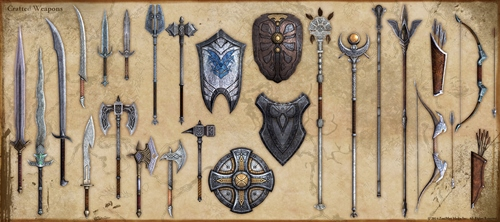
\includegraphics[width=\textwidth]{Equipment.png}
\end{figure}

\section{Combat Techniques}

Combat techniques are special maneuvers that you can perform while in combat, allowing you to do more than just move and swing a weapon. Combat techniques generally require an action to execute and cost stamina. Techniques labeled as "Reaction" can be executed in response to a specific event instead of using an action on your turn. Each reaction technique imposes an additional penalty die on the next one until your next turn. For example, if you have dodged and fought back between turns, attempting to dodge again will be an Acrobatics check with two penalty dice (in addition to any that may be imposed by other circumstances).

\subsection{Common Techniques}

While certain combat techniques will only be available to skilled warriors while wielding specific weapons, some techniques are available to everyone and can be used with various different weapons.

\begin{itemize}
	\item Block (\textit{10 Stamina, Reaction}): If you are targeted by a melee attack, you may attempt to block it. Make an opposed Block check. On a success, you block the attack and take no damage.
	\item Dive for Cover (\textit{Free, Reaction}): When you first notice an enemy, you may dive for the ground as a reaction, preferably behind cover. Otherwise, this technique costs an Action. You are able to cover 10 feet using this move, and you go prone as a result. This move imposes a penalty on ranged attack rolls targeting you.
	\item Dodge (\textit{10 Stamina, Reaction}): If you are targeted by a melee attack, you may attempt to dodge by making an opposing Acrobatics check. On a success, you dodge the opponent's attack entirely and take no damage. On a tie, the dodger wins.
	\item Dual Wield Attacks (\textit{Free, Bonus Action}): If you attack with a light, one-handed weapon and are holding another light, one-handed weapon, you may attack with the latter as a bonus action; however, the second attack does not benefit from your damage bonus. If you use Flurry of Blows while dual wielding, each weapon gets only two attacks, for a total of four. The damage bonus rule still applies to your off-hand weapon in this case.
	\item Fight Back (\textit{10 Stamina, Reaction}): You respond to incoming melee attacks with attacks of your own. You must be within range of the attacker and not otherwise unable to attack. You can only make one attack, it may not be a combat technique. On a success, you avoid coming to harm and your attacker suffers damage. On a tie or failure, your attack fails to land and your attacker successfully strikes you.
	\item Flurry of Blows (\textit{60 Stamina, Action}): You swing your weapon(s) quickly, dealing multiple blows in a single round. Light weapons may attack 3 times, medium weapons may attack twice, and heavy weapons may not use this technique. For the purpose of successive reaction penalty dice, this technique counts as one attack.
	\item Grapple (\textit{20 Stamina, Action}): If you have at least one free hand, you may attempt to grab your target. Make a melee attack using your Athletics skill. You do no damage, but the target is grappled on a success. A grappled target cannot move. Your speed while holding an unwilling creature is halved. A grappled creature may attempt to break free with its action using an opposed Athletics check.
	\item Opportunity Attack (\textit{10 Stamina, Reaction}): If a combatant leaves your melee range during their turn, you may react by making a single attack against them.
	\item Sneak Attack (\textit{Free, Action}): If you are undetected, you may attack a target for bonus damage determined by your Sneak skill (\textit{see section 3.2}). Sneak attacks always gain a bonus die, but their damage multipliers do not stack with those of other combat techniques.
\end{itemize}

\subsection{Weapons \& Skill-Based Combat Techniques}

The following sections describe different types of weapons and the combat techniques associated with that weapon type. Please note that the weapon types listed are merely types and not specific weapons; while all weapons of that type you find in the game will have the listed properties, some features might vary. Also, for every melee technique listed in this section, the following applies: if your target successfully rolls to block your attack and you used a light weapon to make it, the target is recoiled.

\subsubsection{Blade}

Bladed weapons are deadly in the hands of highly skilled wielders thanks to their \textit{Impaling} property. They tend to be more effective against poorly armored opponents thanks to the ease with which blades can cut through flesh compared to the effects of blunt weapons. Bladed weapons in the Elder Scrolls Tabletop RPG come in four varieties:

\begin{itemize}
	\item Daggers (\textit{1d6, Light, One-Handed}): Blades shorter than the forearm. Not very effective against armor, but incredibly deadly in the hands of an adept sneak.
	\item Shortswords (\textit{1d8, Light, One-Handed}): Short, thin bladed swords. More effective than daggers in open combat, but less optimal for sneak attacks.
	\item Longswords (\textit{1d10, Medium, One-Handed}): Long, somewhat heavy blades designed for one- or two-hand grips. Not as quick as a shortsword or dagger, but weighty enough to fare well against armor.
	\item Claymores (\textit{2d6, Heavy, Two-Handed, Reach}): Very long and heavy blades that must be wielded with two hands in order to use them effectively. Great for heavy combat and punching holes in armor at the cost of slow swings.
\end{itemize}

Blade techniques are primarily focused on dealing as much damage as possible. They become available every 25 skill points in Blade as specified in the mastery perk table (\textit{section 3.2}). Each of these techniques costs 60 stamina to execute. If a target successfully blocks a blade technique you made with a medium or heavy blade, they receive recoil. Thus, even failing to land these big hits can come with some benefits. The five blade techniques are:

\begin{itemize}
	\item Power Attack: You wind up and unleash a heavy blow, doubling your damage.
	\item Standing Strike: You plant your feet and strike with all your might, tripling your damage at the cost of being unable to move on the same turn.
	\item Flanking Strike: You swing your weapon broadly across the area in front of you, doubling your damage and allowing you to attack two adjacent targets within reach. (You only roll attack once; each target rolls block/dodge against that number, and attacks are resolved individually.)
	\item Sweeping Attack: You aim low, attempting to strike at your opponent's legs. Damage is doubled; on an extreme success, your opponent is knocked prone.
	\item Dizzying Blow: You swing directly for your opponent's head. Damage is doubled. On an extreme success, your opponent is paralyzed until the end of their next turn.
\end{itemize}

\subsubsection{Blunt}

In general, blunt weapons are more effective against armor due to the manner in which they bludgeon weak points. However, they do not get the \textit{Impaling} bonus to extreme successes; instead, they merely deal max damage. There are four types of blunt weapons:

\begin{itemize}
	\item War Axes (\textit{1d8, Light, One-Handed}): Hand-sized axes, light and quick for blunt weapons. Their weight makes them better at penetrating armor than other light weapons.
	\item Maces (\textit{1d10, Medium, One-Handed}): Bludgeons with a weighty head at the end of a handle. Useful for crumpling skulls and armor alike. Not quite as swift as war axes, but significantly more effective against armored foes.
	\item Battleaxes (\textit{1d12, Heavy, Two-Handed, Reach}): Big, heavy axes that require both hands to swing. Great for cleaving limbs and leaving deep,  grievous wounds.
	\item Warhammers (\textit{2d6, Heavy, Two-Handed, Reach}): Huge hammers intended not for construction but smashing foes. Allows for consistently forceful strikes.
\end{itemize}

Blunt techniques are identical to Blade techniques, except they become available via advancement in the Blunt skill. Again, each technique costs 60 stamina to execute, and if a target successfully blocks one of these attacks made with a medium or heavy weapon, they receive recoil. The five blunt techniques are:

\begin{itemize}
	\item Power Attack: You wind up and unleash a heavy blow, doubling your damage.
	\item Standing Strike: You plant your feet and strike with all your might, tripling your damage at the cost of being unable to move on the same turn.
	\item Flanking Strike: You swing your weapon broadly across the area in front of you, doubling your damage and allowing you to attack two adjacent targets within reach. (You only roll attack once; each target rolls block/dodge against that number, and attacks are resolved individually.)
	\item Sweeping Attack: You aim low, attempting to strike at your opponent's legs. Damage is doubled; on an extreme success, your opponent is knocked prone.
	\item Dizzying Blow: You swing directly for your opponent's head. Damage is doubled. On an extreme success, your opponent is paralyzed until the end of their next turn.
\end{itemize}

\subsubsection{Hand-to-Hand Techniques}

Unarmed attacks deal less damage than blade, blunt and marksman weapons. They do not benefit from the Impaling property, nor do they get to ignore armor points like blunt weapons. They also deal less base damage than any of the listed weapons (\textit{1d4}) and do not have benefit from weapon quality damage bonuses. However, hand-to-hand attacks have the unique benefit of exhausting the target. Whenever you deal damage with an unarmed attack, half of that damage is also removed from the target's stamina. Unarmed attacks also count as light weapons and so benefit from Flurry and dual wielding. Hand-to-Hand techniques are similar to melee weapon techniques, but they are more focused on disrupting the enemy. Like the previous categories, each technique listed here costs 60 stamina to execute.

\begin{itemize}
	\item Power Attack: You wind up and unleash a heavy blow, doubling your damage.
	\item Standing Strike: You plant your feet and strike with all your might, tripling your damage at the cost of being unable to move on the same turn.
	\item Disarming Attack: You strike viciously at your opponent's weapon arm. Your attack deals double damage, and the opponent is disarmed on an extreme success.
	\item Paralyzing Palm: You strike at your opponent's vitals, causing them to reel in pain. Your attack deals double damage, and on an extreme success, the opponent is paralyzed until the end of their next turn.
	\item Power Within: You channel your inner power and strike a powerful blow against your foe. Your damage is doubled. On an extreme success, you may convert half of your damage to fire, frost or shock damage, your choice.
\end{itemize}

\subsubsection{Archery}

Bows are silent and lethal ranged weapons. Bows are often favored by stealthy characters as a way to attack enemies at range with minimal risk of exposure. Their ability to deliver poisons via arrowhead makes them especially potent; even if the arrow does not finish the job, the poison may. While blades can be poisoned and are still highly useful for this purpose, quite a bit of mischief can be caused when one is not within arm's reach. Poisons aside, bows are very precise puncturing weapons. While they are not as effective against armor as blunt weapons, they are highly deadly in the hands of trained archers. All bows in the ESTRPG have the \textit{Impaling} and \textit{Two-Handed} properties, since their arrows are sharp and pointed and bows take both hands to use. Just make sure you bring enough arrows with you! There are two types of bows in the game:

\begin{itemize}
	\item Shortbows (\textit{2d6, 80 ft, Medium}): Bows of modest length, generally allowing for faster draw speed at the cost of less power.
	\item Longbows (\textit{2d8, 150 ft, Heavy}): Bows typically as tall as the archer, with enough power to send arrows flying faster and farther at the cost of slower draw speeds.
\end{itemize}

Marksman attacks in combat use different mechanics from melee attacks; targets cannot react by dodging or blocking. Instead, a difficulty is chosen for the attack roll based on how far away the target is in relation to the weapon's base range (normal for within, hard for within double, extreme for within triple). Bonus and penalty dice are then assigned based on conditions affecting the shot. The conditions are as follows:\\

\begin{tabular}{p{0.3\textwidth}|p{0.3\textwidth}}

Bonus & Penalty\\ \hline
	\begin{itemize}
		\item Aiming
		\item Large target
	\end{itemize}
	&
	\begin{itemize}
		\item Small target
		\item Target is within melee range
		\item Target in partial cover
		\item Target diving for cover
		\item Firing into a melee with friendlies
		\item Fast-moving target (moved 50 feet or more on last turn)
	\end{itemize}\\

\end{tabular}

These apply to ranged attacks with any weapon or spell.

Marksman techniques are less concerned with dealing extra damage and more with improving archery conditions. Nonetheless, they typically do improve upon the already formidable base damage of bows.

\begin{itemize}
	\item Aim (\textit{10 Stamina}): By staying still for a round and taking no damage, you are able to concentrate and line up a good shot. Your next attack has a bonus die and +20 ft to base range.
	\item Volley (\textit{60 Stamina}): You can fire two arrows in one round when using a shortbow.
	\item Trick Shot (\textit{60 Stamina}): Your attack deals double damage and ignores penalty dice imposed by partial cover.
	\item Focus Shot (\textit{60 Stamina}): Your attack deals double damage and ignores penalty dice imposed by firing into a melee.
	\item Snipe (\textit{60 Stamina}): Your attack deals triple damage, and base range is increased by 25\% for this attack. Range bonus does not stack with Aim.
\end{itemize}

Note: You have a limited number of arrows, so be careful with your attacks. It is assumed you are able to recover all your arrows after combat unless something happens to them.

\begin{figure}[H]
	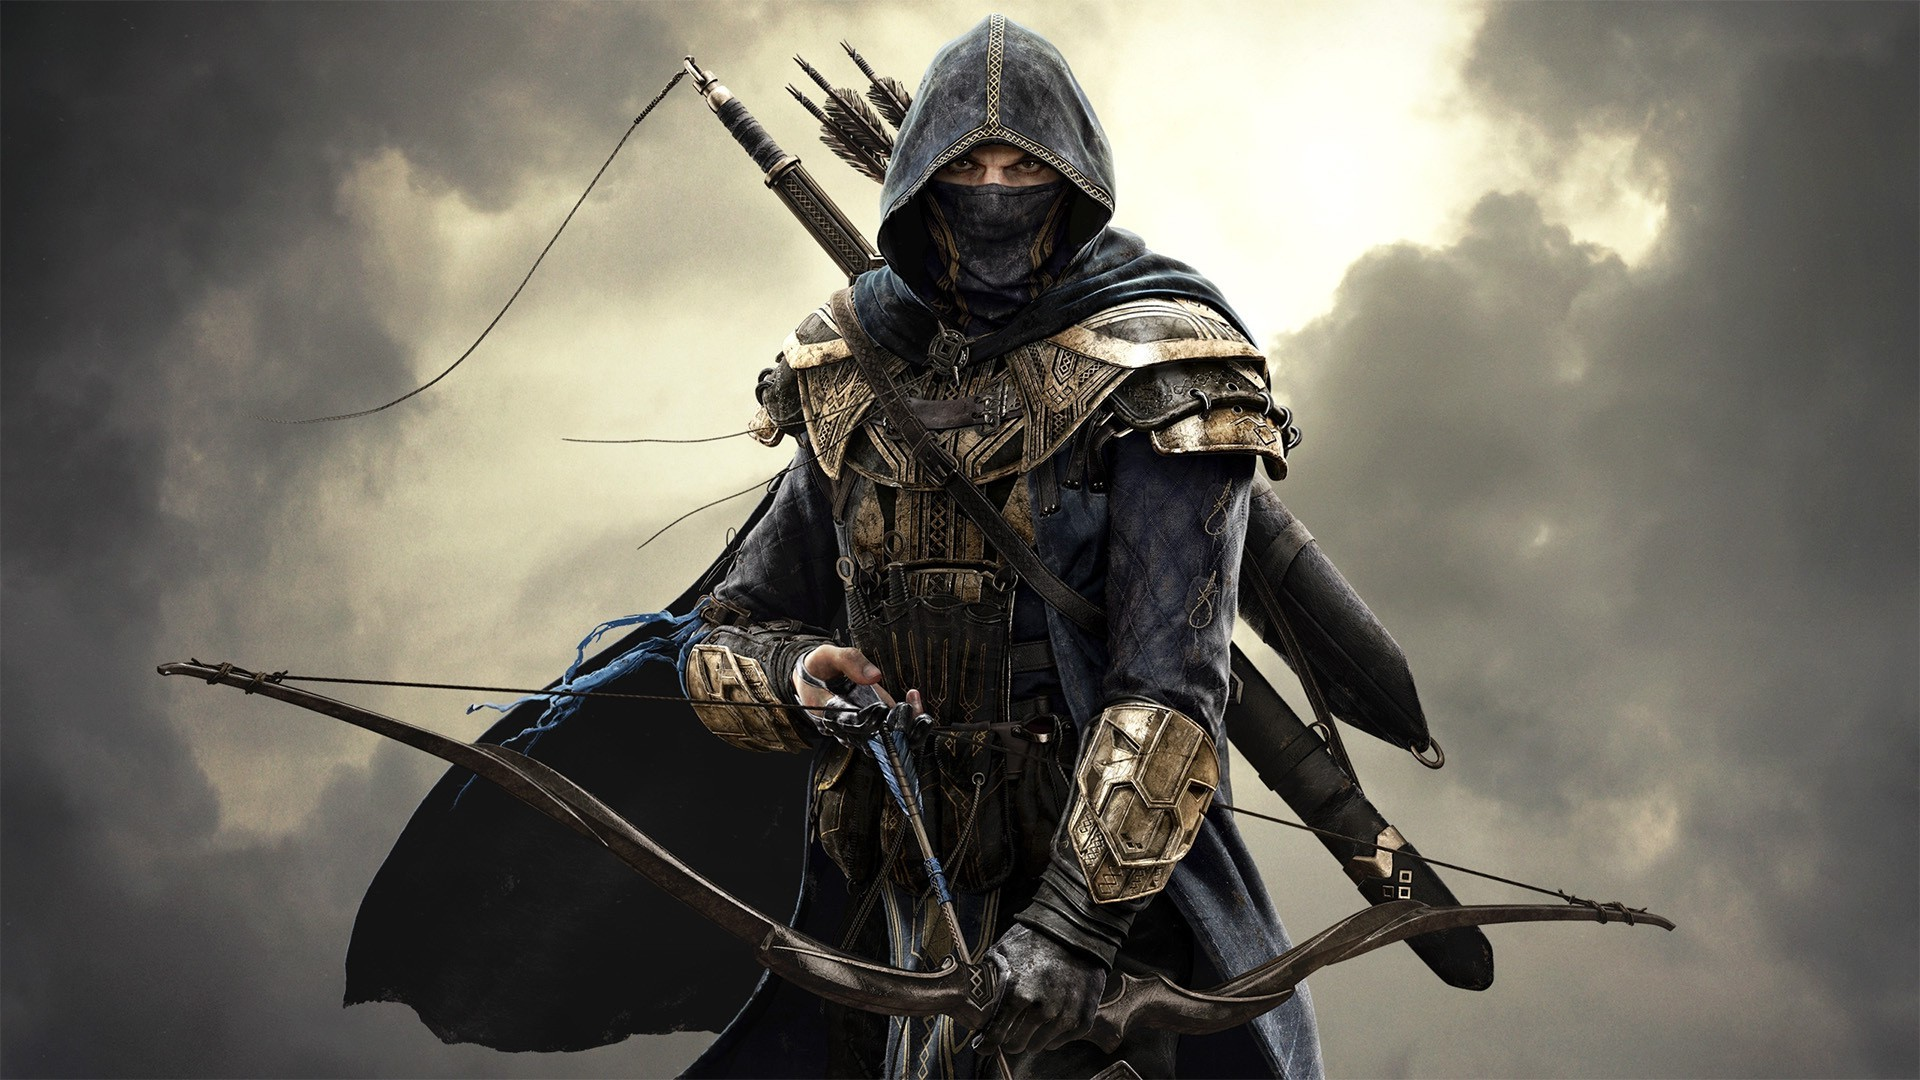
\includegraphics[width=\textwidth]{bretonarcher.png}
\end{figure}

\section{Armors \& Shields}

Armor is quite simple in the ESTRPG. Rather than splitting armor up into various pieces and requiring the player to find them all, armors come in full suits. Each armor has an armor rating. whenever you take physical damage while wearing armor, subtract that armor's rating from the damage. Armor rating does not decrease from attacks unless something special damages the armor.

Armor comes in two varieties: heavy and light. Heavy armor generally provides better protection, but it imposes a penalty die on all non-social Stealth checks. All armor reduces movement speed, but heavy armor tends to reduce it more. Armor penalties can be mitigated by improving your armor skills. Shields are sold separately, but they provide additional armor and a bonus die on block rolls.

\section{Scrolls \& Staves}

Staves have stored spells in them which you can cast without spending magicka. Using one to attack works exactly the same way as using the spell stored in it (see \textit{Chapter 6}), only you do not need to know the spell or be of sufficient level to use it. When a staff runs out of charge, you cannot cast spells with it. It can be recharged by consuming a soul gem or by bringing it to a spell merchant and paying a fee.

Scrolls also allow you to cast stored magic without needing to know the spell, have the skill required to use it or spend any magicka. However, scrolls only allow you to cast a single spell before they are consumed and become completely useless.

\begin{figure}
	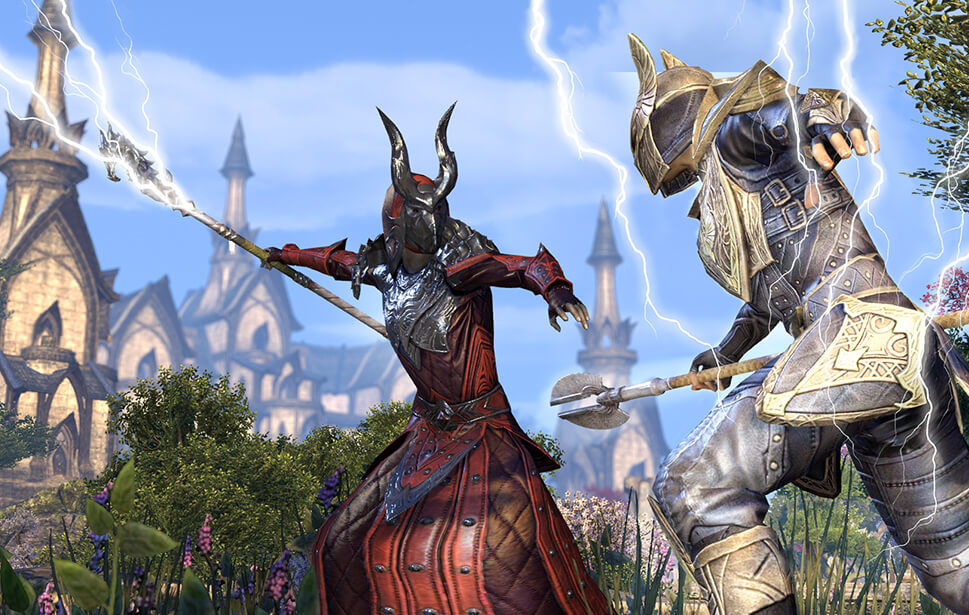
\includegraphics[width=\textwidth]{staves.png}
\end{figure}

\section{Improvised Weapons}
Sometimes, you may find yourself in a fight with no weapons on hand. Some objects may be used as improvised weapons and should be treated as a similar weapon type for the purposes of attacking. A chair leg might be defined as a mace, for example. The GM will decide what stats the item receives in this case. An object that does not resemble a weapon deals 1d6 damage.

\section{Silver Weapons}
You may come across certain creatures who are immune to normal weaponry. Such creatures may have be vulnerable to silver. You can pay a fee of 100 Septims to have a weapon silvered, giving it the Magic property.

\section{Adventuring Gear}
This section lists miscellaneous gear that will be useful in your adventures. Costs listed are \textit{base cost}, which will be modified according to your Mercantile skill.

\begin{itemize}
	\item Acid Vial (25 Septims, 1 lb): A small amount of acid stored in a glass vial. It can be splashed on a target within 5 feet for 2d6 physical damage that ignores armor. Items splashed by acid are damaged.
	\item Alchemical Fire (50 Septims, 1 lb): A flask of sticky fluid that ignites when exposed to air. As an action, you can throw the flask up to 20 feet. Make a Marksman check to hit a creature with the flask. On a hit, the target is ignited and takes 1d4 fire damage at the beginning of each of its turns for the next 3 rounds.
	\item Alchemist's Kit (50 Septims, 2 lbs): contains vials and space to store your potions and alchemy apparatuses.
	\item Alembic (Varying Cost, 7 lbs): Used to distill alchemical mixtures. One of four types of alchemy apparatuses; price varies with quality.
	\item Arrows --- Bundle of 20 (20 Septims, 1 lb): A set of 20 arrows. May be used with shortbows or longbows.
	\item Antitoxin (50 Septims, 1 lb): A potion in a glass bottle. Drink it to cure yourself of poison.
	\item Backpack (20 Septims, 5 lbs): While worn, a backpack allows you to carry an additional 30 lbs of equipment without overencumbering yourself.
	\item Ball Bearings --- Sack of 1,000 (10 Septims, 2 lbs): A sack filled with 1,000 tiny steel balls. You may scatter them in a 5 ft radius; any creature moving through this area that moves more than half its speed must succeed on an Acrobatics check or fall prone.
	\item Bedroll (20 Septims, 7 lbs): Provides sufficient comfort to sleep on hard ground.
	\item Blanket (5 Septims, 3 lbs): Protects you from cold while you sleep.
	\item Block and Tackle (10 Septims, 5 lbs): A set of pulleys, hooks and cables that allows you to hoist objects up to four times the weight you can normally lift.
	\item Book (Varying Cost, 5 lbs): A book containing information that could include lore, illustrations, diagrams or really anything else that can be written down on paper.
	\item Calcinator (Varying Cost, 5 lbs): A metal bowl on a stand, used in alchemical processes. One of four alchemical apparatuses. Cost varies with quality.
	\item Caltrops --- Sack of 20 (10 Septims, 2 lbs): A sack filled with small metal spike traps that always point upward no matter how they are oriented. You may scatter them in a 5 ft diameter; creatures moving more than half their speed must succeed on a hard acrobatics check or cease moving and take 5 physical damage.
	\item Candle (1 Septim, 0 lbs): For one hour, a candle will shed 5 feet of bright light and 5 feet of dim light beyond that.
	\item Case, parchment (10 Septims, 1 lb): A protective case that can hold maps, papers and parchments. No more than 10 sheets.
	\item Chain --- 10 ft (15 Septims, 10 lbs): A chain has 20 hit points. It can be broken by success on an extreme Athletics check.
	\item Climber's Kit (40 Septims, 12 lbs): A kit containing ropes, pitons, boot tips and a harness. Allows you to set up to 2 harness points from which you cannot be moved more than 25 feet, even by falling.
	\item Clothes, Common (5 Septims, 3 lbs): Clothes that would be worn by commoners. Cheap, but do not make much of an impression on the wealthy.
	\item Clothes, Costume (25 Septims, 3 lbs): Clothes specially intended to disguise you. May not hold up to close inspection.
	\item Clothes, Fine (30 Septims, 4 lbs): Clothes worn by people of means.
	\item Clothes, Traveling (10 Septims, 2 lbs): Light, durable clothing favored by people on the move.
	\item Crowbar (15 Septims, 5 lbs): Crowbars give you a bonus die on Athletics checks where strength is required and leverage may be applied.
	\item Fishing Tackle (10 Septims, 4 lbs): A set of fishing equipment, contains all you need to fish in rivers or lakes.
	\item Healer's Kit (30 Septims, 3 lbs): A leather pouch containing bandages, splints and salves. You may use this item to stabilize a dying creature. The kit has 10 uses.
	\item Hourglass (40 Septims, 1 lb): A glass container with sand inside. Turning it over allows sand to flow from one partition of the container to the other at a rate such that when it is complete, an hour will have passed.
	\item Hunting Trap (20 Septims, 25 lbs): A sawtoothed steel ring that snaps shut when activated by a pressure plate in the middle. Creatures that step on the pressure plate must succeed on an Acrobatics check to move away before the trap shuts. Otherwise, they take 1d4 physical damage and lose all movement until they are freed. A creature may attempt to break free using a hard Athletics check.
	\item Ink Bottle (40 Septims, 0 lbs): Used for writing.
	\item Ink Pen (1 Septim, 0 lbs): Also used for writing.
	\item Ladder --- 10 feet (10 Septims, 25 lbs): A pair of poles connected by rungs, allowing one to climb up them easily.
	\item Lamp (15 Septims, 1 lb): Casts bright light in a 15-ft radius and dim light an additional 30 feet. Once lit, it burns for 6 hours on a flask of oil.
	\item Lantern, Bullseye (40 Septims, 2 lbs): A lantern with a single, round opening designed to cast light in a narrow beam. The opening has an attached cover that may be shut. The lantern casts bright light in a 60-ft cone and dim light an additional 60 feet beyond that. Once it, it burns for 6 hours on a flask of oil.
	\item Lantern, Hooded (25 Septims, 2 lbs): Casts bright light in a 30-ft radius and dim light for an additional 30 ft. Once lit, it burns for 6 hours on a flask of oil. As an action, you may lower the hood to change the light level to a 5-ft radius of dim light.
	\item Lock (Varying cost, 1 lb): Locks come with keys and may be used to prevent access to doors or containers. Higher lock difficulties cost more money.
	\item Lockpicks, set of 10 (50 Septims, 1 lb): Allows those skilled in Security to open locks without needing a key.
	\item Manacles (Varying cost, 6 lbs): Metal restraints that can bind a creature of person size or smaller. They can be broken with an extreme Athletics check. Lock levels vary, increasing the price.
	\item Mess Kit (5 Septims, 1 lb): Contains basic utensils and cookware.
	\item Mortar and Pestle (Varying Cost, 1 lb): Essential for creating alchemical mixtures. Higher qualities cost more money.
	\item Oil, flash (3 Septims, 1 lb): A flask containing flammable oil. Useful for fueling lanterns. As an action, you can also splash the oil on a creature 5 feet in front of you or throw it at a creature within 20 feet using a Marksman skill check. A creature covered in oil that takes fire damage will take an additional 5 fire damage. Once they take this extra damage, the oil is consumed. The oil will otherwise dry up after 1 minute. The oil may also be spilled on the ground in a 5-ft radius and lit for 2 rounds, dealing 5 fire damage to anyone who enters the area or ends their turn in the area.
	\item Paper, 1 sheet (1 Septim, 0 lbs): Writing material.
	\item Parchment, 1 sheet (2 Septims, 0 lbs): Finer writing material.
	\item Poison of Illness (15 Septims, 1 lb): A target afflicted by this poison takes 5 damage and the Poisoned condition unless they have poison resistance. The condition lasts 1 round.
	\item Pot, iron (5 Septims, 10 lbs): Useful for more involved cooking than is allowed by a mess kit.
	\item Potion of Healing (50 Septims, 1 lb): A red, sparkling liquid that restores 20 health when drunk.
	\item Pouch (3 Septims, 1 lb): Used to store small items. Expands your encumbrance by 5 lbs.
	\item Quiver (10 Septims, 1 lb): Used to hold up to 20 arrows.
	\item Ram, portable (30 Septims, 35 lbs): Used to break down doors. Gives you a bonus die on Athletics checks made to break structures by ramming into them.
	\item Rations, 1 day (3 Septims, 2 lbs): Contains nonperishable food, enough for one day.
	\item Repair Kit (50 Septims, 8 lbs): Contains all the tools necessary to allow a skilled armorer to repair equipment in the field. Comes with 5 uses.
	\item Retort (Varying Cost, 3 lbs): Used to distill alchemical mixtures. One of four alchemical apparatuses. Cost varies with quality.
	\item Rope --- 50 feet (30 Septims, 10 lbs): Has a multitude of uses for the savvy adventurer. Ropes have 2 health and may be broken out of with a hard Athletics check.
	\item Sack (10 Septims, 1 lb): Used to store items too big for a pouch. Expands your encumbrance by 10 lbs.
	\item Scale (15 Septims, 3 lbs): A set of fine weights, pans and a balance for determining the exact weight of items. Useful for assessing value.
	\item Shovel (5 Septims, 5 lbs): Useful for digging holes in compacted dirt.
	\item Soap (2 Septims, 0 lbs): Used to clean hard surfaces and wash one's body of dirt.
	\item Spyglass (750 Septims, 1 lb): Objects viewed through this glass appear twice as large. Useful for spying and scouting.
	\item Tent (30 Septims, 20 lbs): Big enough to provide shelter for two people. Frustrating to set up.
	\item Tinderbox (10 Septims, 1 lb): Contains flint, fire steel, and tinder used to start a fire. Lighting a torch or anything else with abundant, exposed fuel takes an action; lighting anything else takes 1 minute.
	\item Torch (3 Septims, 1 lb): Sheds bright light in a 20-ft radius and dim light 20 feet beyond that for 1 hour. If used for a melee attack, it uses Blunt and deals 1 fire damage.
\end{itemize}

\begin{figure}[H]
	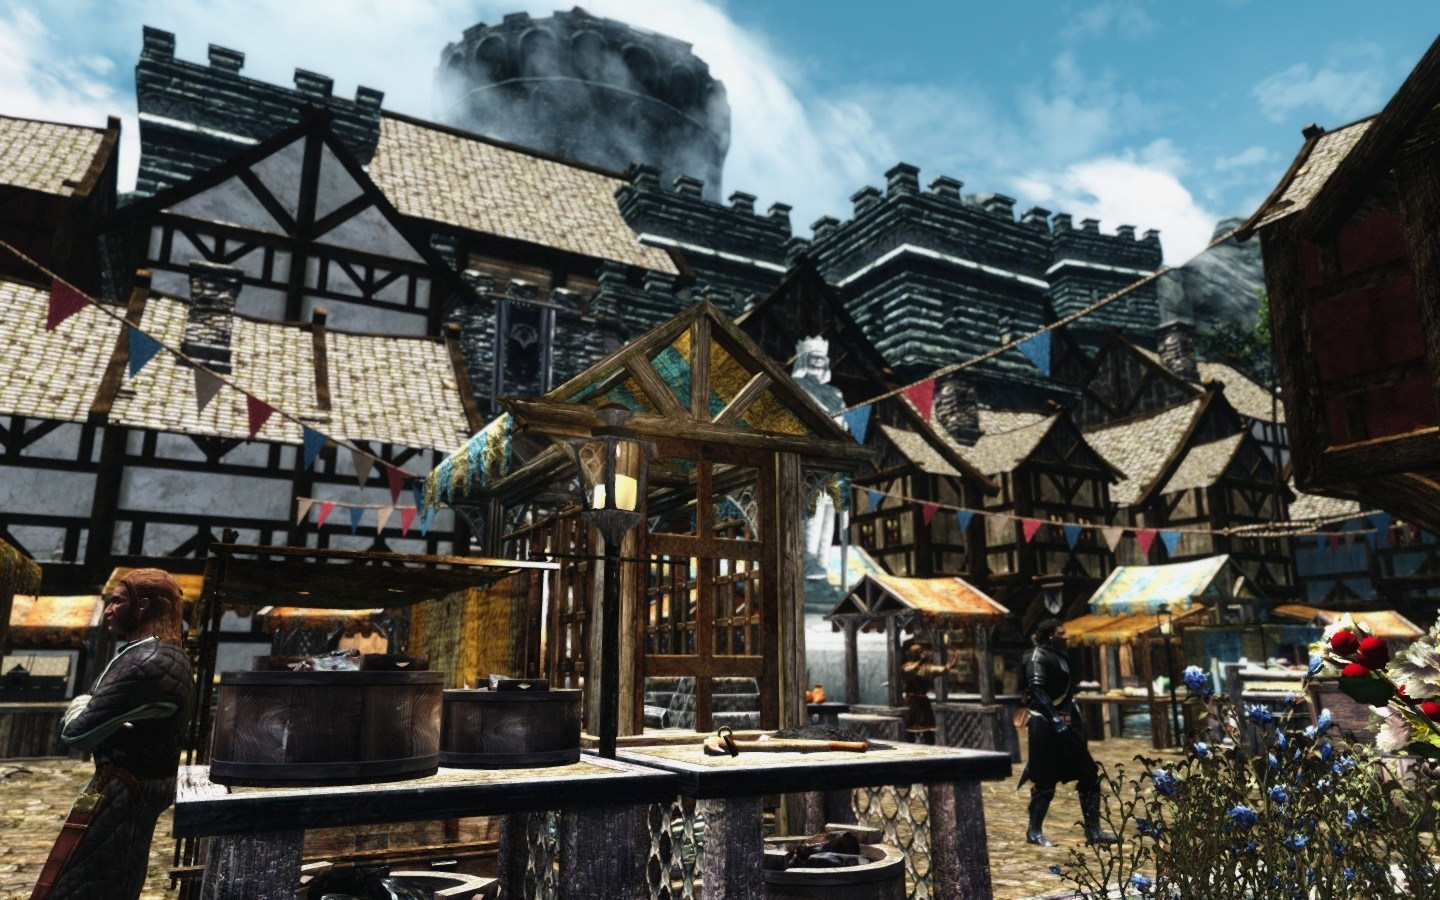
\includegraphics[width=\textwidth]{market.png}
\end{figure}

\chapter{Spellcasting}

\begin{figure}
	\includegraphics[width=\textwidth]{flamespell.png}
\end{figure}

Magic in the Elder Scrolls generally refers to the manipulation of magicka (magical energy) to alter the world in some way. Individual castings of this to achieve effects are known as spells. It can come from many sources, such as starlight, the Divines or Daedric Princes. All the races of Tamriel have some magical aptitude, though those of elvish blood are more naturally gifted.

There are many different forms of magic in Elder Scrolls and they have all been handled differently across the franchise. This game's magic system is based primarily on that from Elder Scrolls IV: Oblivion. Player characters are able to draw on the magicka in their bodies to cast spells, which are governed by the schools of Alteration, Conjuration, Destruction, Illusion, Mysticism and Restoration. Alchemy is also a magic skill in that it involves the manipulation of magical properties in alchemical reagents to create potions and poisons; it will be covered in the next chapter.

Spellcasting is somewhat similar to combat techniques in that it costs points, has the potential to give you greater damage and special effects, and gives you access to gradually more powerful abilities as your skills increase. However, it is different from techniques in that it uses your magicka instead of stamina; spells that deal damage also do not get attribute- or skill-based bonus damage. Spells have static values for their magnitude instead of rolls and so are often more reliable than weapon attacks. Also, increased skill in one of the magic schools reduces the cost of spells in that school, meaning you will have access to far more powerful spells as you level up.

\section{Spellcasting Formulas}

For convenience, here are the max magicka, magicka regeneration and spell range formulas again:

\begin{itemize}
	\item $Magicka=2*Intelligence$
	\item $Range=2*Willpower$
	\item $Regeneration=(5+0.1Willpower)\%$ of max magicka per round
\end{itemize}

\section{Spell Properties}

Each spell costs an action to cast in combat and comes with the following properties:

\begin{itemize}
	\item Effect: What does the spell do?
	\item Target: How the spell's effect is applied (at range, on touch, or on self).
	\item Base Magicka Cost: How much magicka you need to spend to cast this spell.
	\item Magnitude: How big the spell's effect is (e.g. damage dealt, health restored).
	\item Duration: How long the spell's effect lasts.
	\item Area: The radius in which spell effects apply.
	\item School: Which skill is used with the spell.
	\item Skill Level: What skill level is required to cast the spell (Novice, Apprentice, Journeyman, Expert or Master).
	\item Action: Does the spell cost an action, or can it be cast as a reaction or bonus action?
\end{itemize}

Note that not all spells have each property. Most spells do not have an area effect but rather act on a single target, for example. Some spells have multiple effects, each with a different duration and sometimes different targeting styles.

Your skill affects the magicka cost of a spell according to the following formula:

$Cost=Base Cost*(1.4-0.012*Skill)$

Outside of battle or other time-critical situations, magicka costs will be ignored because it is assumed you have enough time to regenerate your magicka reserves. If you are ambushed or otherwise threatened immediately after casting a spell outside of battle, the GM may rule that you must deduct the spell cost from your current magicka in the first round. Also, casting outside of combat still requires that you have enough max magicka to cast the spell, and skill requirements still apply.

\subsection{Spell Attacks}

If the target of your spell is unwilling, you will have to make a spell attack roll. Touch spells count as melee attacks, and ranged spells count as ranged attacks; both categories are affected by the bonus and penalty conditions that might normally affect an attack roll. In order to make the attack roll, make sure your target is within range and roll against the skill that governs the spell. If you are successful, the target is hit and the spell takes effect.

If you have a free hand, you may cast another spell of Apprentice level or lower as a bonus action. You must have the magicka to do so, and you must make a spell attack roll if applicable. All the normal rules for spellcasting apply.

Note that spells make noise when cast and so are difficult to use undetected. Journeymen of Illusion may cast any spell silently.

\section{Schools of Magic}

Mainstream culture in Tamriel recognizes six schools of magic, each concerned with different magical effects. Beginning the game with a school of magic as a major skill will grant you starting skills from that school. All classes with magic for at least one major skill begin the game with the following spells in addition to those granted by the schools:

\begin{itemize}
	\item Flare (\textit{11 Magicka, Ranged, Destruction Novice}): The target takes 6 points of fire damage and an additional 1d4 on its next turn.
	\item Heal Minor Wounds (\textit{14 Magicka, Self, Restoration Novice}): You recover 8 health.
\end{itemize}

In combat, casting a spell requires an action unless otherwise specified.

\subsection{Alteration}

The school of Alteration covers spells that manipulate the natural world and its physical properties. Alteration magic allows you to do things like resist physical and elemental attacks, change the weight of items, open locks, and breathe underwater. Some Alteration spells target opponents with negative effects, requiring a spell attack roll.

If Alteration is one of your major skills, you begin the game with the following spells:
\begin{itemize}
	\item Open Very Easy Lock (\textit{7 Magicka, Ranged, Novice}): Automatically opens a lock of Very Easy difficulty.
	\item Protect (\textit{10 Magicka, Self, Novice}): +1 to your current armor rating for 5 rounds. You may cast this spell as a bonus action.
\end{itemize}

On an extreme success, Alteration attacks may have greater magnitude or duration.

\newpage
\subsection{Conjuration}

\begin{wrapfigure}{L}{0.35\textwidth}
	\includegraphics[width=\textwidth]{conjurer.png}
\end{wrapfigure}

The school of Conjuration is used primarily to summon things from Oblivion. It can be used to conjure daedra and undead as well as summon daedric weapons and armor for very brief periods of time. Summoned creatures will act independently, but are allied with you. They may respond to commands if they are intelligent. You can only have one summoned minion at once. If you conjure a new minion before the current one's time runs out, the current one is dismissed. If you attack your minion, it will become hostile.

If Conjuration is one of your major skills, you begin the game with the following spells:
\begin{itemize}
	\item Summon Skeleton (\textit{45 Magicka, Self, Apprentice}): Summons a Skeleton minion for 7 rounds.
	\item Turn Undead (\textit{11 Magicka, Ranged, Novice}): Undead up to level 3 must use their turn to move as far from you as possible as long as they can see you, and they cannot attack you. This effect lasts until the end of the target's third turn.
\end{itemize}

\subsection{Destruction}

The school of Destruction involves all spells that directly harm the body, possessions or abilities. Destruction spells can be used to project flames, ice or lightning as well as break armor, fatigue combatants, and much more. Destruction spells almost always require a spell attack roll.

If Destruction is one of your major skills, you begin the game with the following spells:
\begin{itemize}
	\item Cold Touch (\textit{23 Magicka, Touch, Novice}): The target takes 15 points of frost damage and 7 points of stamina damage.
	\item Shocking Touch (\textit{14 Magicka, Touch, Novice}): The target takes 10 points of shock damage and 5 points of magicka damage.
\end{itemize}

On an extreme success, elemental damage spells get a bonus effect. Fire spells set the target on fire, dealing an additional 10\% fire damage over the course of the target's next three turns (damage is taken at the beginning of each turn). Frost spells root the target in place with ice, preventing them from moving on their next turn unless they succeed on a hard Athletics check. Shock spells jump to a nearby target within range, dealing the same effect on the new target.

The following are special abilities you gain access to at certain skill levels (see the mastery perk chart, section 3.2):

Dual Casting: If you have two free hands, you can dual cast any destruction spell. Dual casted spells require double the magicka cost, but they deal triple damage.

Elemental Mastery: Choose an element: fire, frost or lightning. From now on, all spells that deal that damage type gain the corresponding effect:

\begin{itemize}
	\item Fire: Enemies under 20\% health are inflicted with fear for 3 turns when struck by a fire spell.
	\item Frost: Enemies under 20\% health are paralyzed for 3 turns when struck by a frost spell.
	\item Lightning: Enemies under 15\% health are immediately turned into ash when struck by a shock spell.
\end{itemize}

You may only choose one element to master, and you choose it once you achieve the mastery perk. The effects of this perk do not take effect on enemies that are resistant to that element, defined as having a resistance greater than 0.

\subsection{Illusion}

Illusion spells manipulate the senses and emotions of their targets. Illusion is useful both in and out of battle with effects such as charms, invisibility, muffling, calming, frenzy and courage. Some illusions will require spell attack rolls. People usually do not like to be tricked with illusions, so using them in social situations will require subterfuge. Illusionists must be clever!

If Illusion is one of your major skills, you begin the game with the following spells:
\begin{itemize}
	\item Soothing Touch (\textit{13 Magicka, Touch, Novice}): Targets up to level 2 are calmed for 2 rounds. Calmed targets will not move or perform any actions. They are aware of your presence, and the effect will end if you attack them.
	\item Starlight (\textit{14 Magicka, Self, Novice}): You emanate bright light in a 20 ft radius and dim light in a 40 ft radius for 1 minute. You may cast this spell as a bonus action.
\end{itemize}

On an extreme success, Illusion attacks may have increased magnitude or duration.

\subsection{Mysticism}

The school of Mysticism is concerned with unraveling the mysteries of the world. Spells under this school are grouped less by categorical membership characteristics and more by tradition, as these spells were considered a single school by the Psijic Order, a group of mages who created them. Effects in this school allow you to detect living creatures, dispel, reflect or absorb magical effects, harvest souls for enchanting, and move distant objects. Some Mysticism spells target opponents and will require attack rolls.

If Mysticism is one of your major skills, you begin the game with the following spells:
\begin{itemize}
	\item Minor Dispel (\textit{22 Magicka, Self, Novice}): For all magical effects currently active on you, those that were imposed by a spell that cost no more than 40 magicka are immediately ended. Applies to beneficial and harmful spells alike. Does not apply to magical effects imposed by abilities, diseases, curses, enchantments, potions, poisons or scolls.
	\item Minor Life Detection (\textit{15 Magicka, Self, Novice}): For the next 12 seconds, all living creatures within 60 feet of you appear to give off a faint purple glow that you can see through solid objects. Only you can see this effect.
\end{itemize}

On an extreme success, Mysticism spells may have increased magnitude or duration.

\subsection{Restoration}

\begin{figure}[H]
	\includegraphics[width=\textwidth]{healing.png}
\end{figure}

Restoration magic involves all spells which heal, rest, cure, restore or fortify a target. The effects of Restoration are many and varied, and they include things such as restore health, restore stamina, fortify health, stamina and magicka, fortify skills and attributes, cure poison and diseases and resist magicka. A few Restoration spells can act as attacks, though not many.

If Restoration is one of your major skills, you begin the game with the following spell:
\begin{itemize}
	\item Absorb Health (\textit{12 Magicka, Touch, Novice}): Transfer 5 health from the target to you.
	\item Minor Healing Hands (\textit{32 Magicka, Touch, Apprentice}): Heals the target for 15 health.
\end{itemize}

On an extreme success, Restoration spells may have increased magnitude or duration.

\section{Learning New Spells}

In the Elder Scrolls, there is no limit on how many spells you can know. You can learn new spells by finding spell vendors in towns or in Mages Guild buildings, reading spell tomes, or even crafting your own spells if you can gain access to a rare spellmaking altar.

\subsection{Spellmaking}

If you have access to a spellmaking altar, you can make your own spells. Such altars are exceedingly rare; for example, the only spellmaking altars in Cyrodiil are found at the Arcane University of the Imperial City, which can only be accessed by Mages Guild affiliates who have undergone a certain level of training. Once you have acquired access, however, use the following rules to create a spell:

\begin{itemize}
	\item You get to choose the spell's name.
	\item To give the spell a certain effect, you must already know a spell with that effect. This includes race and birthsign powers.
	\item Multiple effects may be added to a single spell.
	\item For each effect, you choose the targeting type, magnitude, duration and area.
	\item Calculate the magicka cost using the following formula: $Total Cost=0.1Base Cost*0.15Area*Duration*Magnitude^{1.28}$
\end{itemize}

If the spell is ranged, multiply the result by 1.5 to get the final base cost. Duration is in rounds. Ask your GM for information on the base costs of effects or use the following link: \url{http://en.uesp.net/wiki/Oblivion:Spell_Effects}

Once you have these things determined, you must perform a 2-hour ritual to create the spell. The materials for the ritual cost a total of three times the magicka cost of the spell.

\chapter{Crafting}

The Elder Scrolls franchise has featured a number of different crafting systems that allowed you to create weapons, armor, potions, poisons, spells, and enchantments. This chapter is dedicated to describing the crafting systems of the Elder Scrolls Tabletop RPG: Alchemy, Blacksmithing and Enchanting. These all require some calculation, so be sure to have those calculators handy! Fortunately, you will not be doing them often. (Spellmaking is covered in Chapter 6. See section 6.4.1. for details.)

\section{Alchemy}

(Please note: Alchemy is indisputably the most calculation-intensive crafting skill thanks to Bethesda's convoluted system! I have simplified it somewhat, but it still requires you to pay careful attention every time you craft a potion! You've been warned!)

Alchemy is the art of making potions and poisons. Many substances have latent magical properties that only come out when properly distilled. To create alchemical concoctions, you need a mortar and pestle and at least two ingredients to mix together. You can mix up to four ingredients at once. If two of the ingredients share a property, the resulting mixture will have that property as well. Using more than two ingredients with the same effect will not increase the magnitude or duration of that effect, however; these are determined by skill level and the alchemy equipment you use.

This method can be used to discover the properties possessed by the reagents you use. You can also eat a small portion of a single ingredient to learn that ingredient's most prominent properties. This is called \textit{wortcraft}. As your Alchemy skill improves, your wortcraft will allow you to detect more properties from individual reagents. You may also learn some alchemical properties from recipes or books. Seek out your local alchemist for more information. It is recommended you keep an alchemy notebook detailing the known properties of reagents.

\subsection{Potion or Poison?}

In the Elder Scrolls series, some factor determines whether your alchemical concoction qualifies as a potion or a poison, which affects whether you drink it or apply it to your weapon when used. The factor varies by game. In the Elder Scrolls Tabletop, there is no hard difference between potions and poisons. In fact, any concoction can be drunk or applied to a weapon if you wish. You could drink a Damage Health poison or apply a Restore Health potion to an arrow if you really wanted to.

\subsection{Alchemy Apparatuses}

While the mortar and pestle is the only alchemy apparatus you need to craft a potion, there are other types of apparatuses you can use to improve upon its effects. Each type comes in five quality levels, the use of which is restricted by current Alchemy level: Novice, Apprentice, Journeyman, Expert and Master. Each quality level has a value used in the alchemy equations. The following values apply to each apparatus:

\begin{itemize}
	\item Novice: 0.1
	\item Apprentice: 0.25
	\item Journeyman: 0.5
	\item Expert: 0.75
	\item Master: 1
\end{itemize}

\newpage
\subsubsection{Mortar and Pestle}

\begin{wrapfigure}{R}{0.2\textwidth}
	\includegraphics[width=\textwidth]{mortarpestle.png}
\end{wrapfigure}

This apparatus consists of a hard bowl made of stone, ceramic or hard wood (the mortar) and a heavy, blunt, club-shaped object (the pestle). Reagents are placed into the mortar and then ground into a fine mixture which is then stirred into water to create a potion. The mortar and pestle are required to craft any potion or poison.

The magnitude and duration of each effect of mixtures produced using only a mortar and pestle are called the \textit{base magnitude} and \textit{base duration}. These are used as intermediate values when other apparatuses are involved; otherwise, they are the true magnitude and duration of the mixture. Base magnitude and duration are calculated with the following formulas:

\begin{itemize}
	\item $Base Magnitude=(\frac{Alchemy Skill+25MortarPestleQuality}{0.4EffectBaseCost})^{1/2.28}$
	\item $Base Duration=4*Base Magnitude$
\end{itemize}

Certain potion effects do not come with a magnitude, such as water breathing. Dispel effects likewise do not come with a duration. For these special cases, use the following formulas instead:

\begin{itemize}
	\item $Base Magnitude=(\frac{Alchemy Skill+MortarPestleQuality*25}{0.1EffectBaseCost})^{1/1.28}$
	\item $Base Duration=\frac{Alchemy Skill+MortarPestleQuality*25}{0.1EffectBaseCost}$
\end{itemize}

(Author note: I am not sure whether the exponent difference is a typo or not. If your potion magnitude seems off, try using the other exponent and see if it makes more sense. Let me know if this comes up in game.)

The value \textit{MortarPestleQuality} is taken from the list in the previous subsection. The value used for \textit{Effect Base Cost} comes from which types of effects the potion will have. Ask your GM for the value needed or consult the following link: \url{http://en.uesp.net/wiki/Oblivion:Spell_Effects}

\newpage
\subsubsection{Retort}

\begin{wrapfigure}{L}{0.2\textwidth}
	\includegraphics[width=\textwidth]{retort.png}
\end{wrapfigure}

A retort is a roughly spherical vessel with a long, downward-pointing neck. It is typically made of glass, though it may also be made of metal. Retorts are used to distill liquids by allowing vapors to condense in the neck, after which they flow downward into a collection vessel placed underneath.

If you use a retort in your concoction, it will increase the magnitude and duration of all positive effects. Magnitudes are increased by $50\%*Quality$. Durations are increased by $100\%*Quality$.

\subsubsection{Calcinator}

\begin{wrapfigure}{R}{0.2\textwidth}
	\includegraphics[width=\textwidth]{calcinator.png}
\end{wrapfigure}

A calcinator is a metal bowl on a ring stand. An alchemical mixture is placed into it above an open flame, heating it to temperatures at which some compounds in the mixture decompose or transition into other forms.

Using a calcinator in your concoction will increase the magnitude and duration of both positive and negative effects. The magnitude and duration of positive effects are increased by $35\%*Quality$, and the magnitude and duration of negative effects are increased by $140\%*Quality$.

\subsubsection{Alembic}

\begin{wrapfigure}{L}{0.3\textwidth}
	\includegraphics[width=\textwidth]{alembic.png}
\end{wrapfigure}

An alembic consists of two glass vessels joined by a downward-sloping tube. The mixture is heated in one vessel, producing vapors which collect at the top of the tube and flow into the collection vessel. The only difference between this and a retort is that the retort has the tube joined with the top of the heated vessel, suggesting the game developers did not think thoroughly about their choice of alchemy apparatuses. In fact, retorts are often part of an alembic.

Regardless, using an alembic will increase the magnitude and duration of your mixture's negative effects. Magnitudes are increased by $50\%*Quality$. Durations are increased by $100\%*Quality$.

\subsubsection{Using Multiple Apparatuses}
When you use multiple apparatuses in a potion, the modifying percentages are added before being applied to the base magnitude and duration. For example, a positive effect will increase by 240\% when a master retort and calcinator are used.

\subsubsection{Selling Potions}
Potions are often a great way of making money. The base cost for each potion you make is equal to $0.45(Alchemy Skill*25MortarPestleQuality)$.

\section{Blacksmithing}

The Elder Scrolls V: Skyrim was the first entry in the franchise to introduce a crafting system for weapons and armor. In previous titles, the Armorer skill was only used to repair items. Since the Elder Scrolls Tabletop is primarily based on the mechanics of Morrowind and Oblivion, the blacksmithing system is made from scratch to provide a simple, sensible way to create weapons and armor.

\begin{figure}[H]
	\includegraphics[width=0.65\textwidth]{blacksmith.png}
\end{figure}

\subsection{Requirements}
Unlike in Skyrim, the Elder Scrolls Tabletop does not require that you collect a set of components necessary to craft an item. Rather, the GM will specify a gold cost for crafting the item which is assumed to cover the expenses of acquiring the components. Blacksmithing can be very expensive!

Certain narrative conditions may be required before you can craft an item. Does your character have the knowledge needed to smith with a certain material or in a certain style? Are you able to find or purchase all the materials you need, or are some items completely unavailable? Sometimes, narrative conditions can reduce the cost of crafting an item as well. For example, if you collected a lot of Dwemer metal while exploring a Dwemer ruin, crafting Dwemer metal items should not cost as much. Work with your GM to decide the conditions affecting your ability to create items.

When you have met all conditions, you need access to a forge and enough time to work. Don't expect to craft items in a dungeon.

\section{Enchanting}

Enchanting is the art of applying persistent magical effects to items. Enchanted items are highly sought after by most cultures in Tamriel for a multitude of reasons. For example, their effects are constant and do not drain magicka when used, they can be used by people without magical training and they are immune to dispel effects. Weapons with enchantments have a limited number of charges, though they may be recharged by spell merchants or by using filled soul gems. Enchanted weapons also gain the Magic property, even when their enchantment charges are depleted. Beware, however: blacksmiths cannot repair enchanted items unless their Armorer skill is Journeyman level or higher.

\subsection{Requirements}
To begin enchanting, you must first gain access to an enchanting altar. These are significantly more common than spellmaking altars and may be found in places such as Mages Guild buildings or wizards' homes. Once you have access to an enchanting altar, you need a soul gem with a trapped soul and an item to receive the enchantment. You may place any magical effect on the item if it is the effect of a spell you know and can cast. You also get to name the item. Certain spell effects cannot be used as enchantments. For example, worn items cannot be enchanted with healing effects. Spell effects may be denied for enchantment at the GM's discretion.

With all these things, you may perform a one-hour ritual to carry out the enchantment. Various other components are needed, the cost of which is equal to the base effect cost (ask your GM or see \url{http://en.uesp.net/wiki/Oblivion:Spell_Effects}) times the magnitude of the effect. Only one effect can be placed on an item at a time. If you perform the enchantment ritual on an item that is already enchanted, its enchantment is overwritten by the new one. The base value of an enchanted item increases by the magnitude of the effect multiplied by the effect's barter factor (see \url{http://en.uesp.net/wiki/Oblivion:Spell_Effects}).

\subsection{Soul Gems}

Soul gems are special magic crystals that can be used to capture the souls of living creatures when they die. Once filled, they can be used to apply enchantments or recharge enchanted items. Soul gems come in six quality levels:

\begin{itemize}
	\item Petty
	\item Lesser
	\item Common
	\item Greater
	\item Grand
	\item Black
\end{itemize}

Creature souls come in five sizes that correspond with soul gem types: Petty, Lesser, Common, Greater and Grand. A soul gem can hold souls of equal or lesser size. The souls of intelligent creatures (humanoids and the like) always count as Grand, but they may only be stored in black soul gems. This practice is illegal and is considered a form of necromancy. Nevertheless, it is possible.

\begin{wrapfigure}{L}{0.37\textwidth}
	\includegraphics[width=\textwidth]{soulgem.png}
\end{wrapfigure}

Capturing a soul is quite simple: if the target dies while affected by a Soul Trap effect and you have a soul gem capable of holding its soul, you may choose to fill the soul gem with it. Soul Trap effects can be applied by spells or even enchanted weapons.

When a soul gem is used for enchanting or recharging, the crystal breaks and cannot be reused. A soul gem with a soul inside cannot contain another soul, nor can the trapped soul be discarded and replaced.

\subsection{Weapon Enchantments}
Weapon enchantments have a certain amount of magicka stored in them and expend a certain amount of magicka each time they are used. The amount of magicka spent is determined by the spell cost formula described in section 6.4.1; it depends on magnitude and effect. You get to choose the magnitude of the enchantment you place on a weapon so long as the resulting cost does not exceed 85. The maximum amount of magicka stored in a weapon enchantment is determined by the level of the soul used to enchant the item. The magicka value of each soul level is as follows:

\begin{itemize}
	\item Petty: 150 magicka
	\item Lesser: 300 magicka
	\item Common: 800 magicka
	\item Greater: 1200 magicka
	\item Grand: 1600 magicka
\end{itemize}

Therefore, the number of uses is determined by the charge of the item divided by the magicka cost of the effect. A maximum magnitude enchantment made with a grand soul would therefore have 18 charges, for example. 

Whenever you use a soul to recharge an item, it regains magicka equal to the size of the soul used. For example, a weapon with a charge of 1000/1600 that is recharged with a petty soul will end up with 1150/1600 magicka.

\subsection{Worn Enchantments}
Enchantments can also be placed on clothing, jewelry and armor. Worn enchantments do not expend charge but rather have a constant effect that is always active so long as you are wearing the item. The effect magnitude of worn item enchantments cannot be chosen, but is rather a product of the soul level used to create it. To determine the magnitude of the enchantment, ask your GM or consult the table at \url{http://en.uesp.net/wiki/Oblivion:Enchanting#Worn_Enchantments}.

\begin{figure}
	\includegraphics[width=\textwidth]{Enchanting.png}
\end{figure}

\chapter{Adventuring and Downtime}
This chapter covers rules about adventuring and what goes on between adventures.

\section{Leveling Up}
When your GM decides you have enough experience and you have time to rest, you main gain a level. You get the following benefits:

\begin{itemize}
	\item Your max health increases by 10\% of your Endurance.
	\item You may distribute 10 points among your major skills, but no more than 5 into any single one.
	\item You may distribute 10 points among your minor skills, but no more than 3 into any single one.
	\item Once your skill points are distributed, select three primary attributes to increase. This is where the governing attributes of skills come in: if you have not raised any skills governed by an attribute, a selected attribute will increase by only one point. If you have put 1-4 points into skills governed by that attribute, it increases by 2 points. If you have put 5-7 points in skills governed by that attribute, it increases by 3 points. If you have put 8-9 points in skills governed by that attribute, it increases by 4 points. Finally, if you have put 10 or more points into skills governed by an attribute, it increases by 5 points.
\end{itemize}

Example: Ingvar Iron-Fist the Nord Barbarian increases his level from 1 to 2. His Endurance is 55, so his max health increases by 5 points. He puts 4 skill points into Blunt, 2 into Athletics and 4 into Light Armor for his major skills. For his minors, he puts 3 into Acrobatics, 3 into Sneak, 3 into Marksman and 1 into Speechcraft. He selects the attributes Strength, Speed and Endurance to increase. He has put 4 points into Strength skills, so his Strength goes up by 2 points. He has put 10 points into Speed skills, so his Speed goes up by 5. He has put no points into Endurance skills, so his Endurance goes up by 1.

\section{Encumbrance}
You are able to carry a weight equal to $5*Strength$ in pounds. If you exceed this weight, you are encumbered and cannot move. Mounts do not have this limitation, but don't get crazy. There are also spells which can alter encumbrance limits.

\section{Travel}
Characters can travel 24 miles per day, assuming they are traveling for a full 8 hours. Each additional hour of travel after that risks exhaustion. Make a percentile roll at the end of each additional hour. You must roll less than or equal to $50-5*extra hours$ or increase your exhaustion level.

Mounts are able to move double speed for one hour, but they must rest an hour before they can do so again. Vehicles are limited by specific speeds, but they may be able to travel for over 8 hours a day without penalty.

Difficult terrain halves travel speed while it is traversed.

\begin{figure}[H]
	\includegraphics[width=\textwidth]{Morrowind.png}
\end{figure}

\section{Resting}
A short rest is defined by a period of at least an hour during which time you do nothing more strenuous than eat, drink, tend to wounds or other physically restful tasks. Your health, magicka and stamina are fully recovered after short rest, though you may not decrease your level of exhaustion. If you have enough experience, you may gain a level during this time.

A long rest is a period spanning at least 8 hours of sleep and light activity including no more than 2 hours of standing watch. You gain all the benefits of a short rest and may decrease your exhaustion by one level. You must complete a long rest once per day with access to sufficient food and drink or else your exhaustion will increase a level.

\section{Survival}
Survival in the Elder Scrolls Tabletop relies on a combination of roleplaying and skill checks. There are no "Surivival" skills like there are in other RPGs; rather, the effects of what you do will be decided by which actions you take and what skills you character possesses. Alchemy, for example, may be useful to determine whether plants are safe for eating. Sneak may be useful to hunt for food. Acrobatics could be useful to get to a vantage point and find running water. Improvise, and wilderness survival will still be a fun challenge.

\subsection{Food}
A grown humanoid needs a pound of food a day to survive. Eating half a pound of food in a day will count as a half-day without food. You can go without food for a number of days equal to $3+0.05Endurance$. After this point, each full day you go without food will increase your exhaustion by one level. A normal day of eating resets the count.

\subsection{Water}
A character needs a gallon of water a day, or two if the weather is hot and dry. Characters who only drink half that in a day must roll less than or equal to $75-0.05Endurance$ or suffer a level of exhaustion. Characters who get even less gain an exhaustion level automatically. If the character already has at least one exhaustion level, they gain two exhaustion levels due to lack of water.

\section{Vision}
Most tasks require vision to some extent. \textit{Lightly obscured} areas provide a bonus die to Sneak checks. \textit{Heavily obscured areas} obstruct vision entirely imposing blindness on everyone in them. Certain weather conditions may obscure vision. Bright light does not obscure, dim light obscures lightly, and darkness obscured heavily. Vision-altering effects may change how light levels affect your character.

\section{Lockpicking}
Picking locks depends on your Security skill. As long as you have a lockpick, you can attempt to pick a lock. You can automatically pick locks at your skill level as defined in the mastery perk chart. You may attempt to pick higher level locks, but you must roll to succeed. If the lock is one level higher than your automatic success level, you need a normal success. If the lock is two levels higher, you need a hard success. If the lock is three levels higher, you need an extreme success. If the lock is four levels higher, it is impossible.

\section{Traps}
You're likely to encounter traps whenever you venture into a dungeon. Detecting traps works using two skills: Sneak and Security. Having a high Sneak skill allows you to set well-hidden traps since you know a lot about hiding things from sight. Security is used to detect the presence of traps and successfully disarm them. Thus, attempting to set traps for other characters will rely on your Sneak and attempting to detect traps before you run into them will depend on your Security.

\section{Different Types of Movement}

\subsection{Climbing and Swimming}
While climbing or swimming, each foot moved costs an extra foot of your movement (or an extra 2 feet in difficult terrain). If conditions are especially hostile, you may be required to make an Athletics or Acrobatics check.

\subsection{Jumping}
If you have at least 10 feet to get a running start, you can long jump a distance in feet equal to one-fifth of your Acrobatics or Strength, whichever is higher. Standing long jumps can only cover half that distance. Each foot you clear costs a foot of movement. You may be required to make an Acrobatics check to jump farther than you normally can.

If you have at least 10 feet to get a running start, you can high jump a height in feet equal to 3+5\% of your Acrobatics or Strength, whichever is higher. Standing high jumps can only jump half as high. You may be required to make an Acrobatics check to jump higher than you normally can. You can extend you arms to reach higher while jumping.

\subsection{Falling}
Gravity exists in the world of Elder Scrolls, and you will get hurt if you fall down. Experienced acrobats are able to handle falls better than the average person, however. For every 10 feet you fall, you suffer 4d20 health damage, ignoring armor. For every 25 points in your Acrobatics skill, this distance increases by 5 feet.

\section{Social Interaction}
Your Personality attribute along with various factors will set an NPC's initial disposition toward you. Rather than rolling Speechcraft to determine whether an NPC is convinced of specific things, Speechcraft checks allow you to increase your disposition with an NPC by varying amounts depending on your level of success. The resulting disposition level may be high enough that the NPC is willing to give you something you ask for, depending on what it is.

The limits on Speechcraft checks depend on your roleplaying: you may not attempt a roll for the same oratory tactic twice in the same conversation. You also cannot make more than three Speechcraft checks to improve disposition in a single conversation, meaning you must take time to build up a positive rapport with an NPC unless you are very skilled or lucky. Speechcraft mastery perks improve your ability to do this.

NPC disposition may be affected by circumstance. If you cannot improve disposition well enough in a single conversation, you might try doing something that the NPC will like. Gifts of money or valuable items will help as well, but be sure to give a gift appropriate to the NPC's wealth and station, or else they may find it insulting!

\section{Downtime}

\subsection{Lifestyle Expenses}
Between adventures, you need to pay the expenses demanded by your lifestyle. It is up to you what sort of lifestyle you wish to live, so long as you can afford it. This has no mechanical effect, but it may change how NPCs are disposed to react to you. The local nobility might give you more attention if you are known to live a wealthy lifestyle. Lifestyle costs:

\begin{itemize}
	\item Wretched (Inhumane): 0 Septims/day
	\item Squalid (Basic shelter): 10 Septims/day
	\item Poor (Sufficient but unpredictable): 25 Septims/day
	\item Modest (Stable home): 100 Septims/day
	\item Comfortable (Middle-class): 200 Septims/day
	\item Wealthy (Good businessman): 500 Septims/day
	\item Aristocratic (Old money): At least 1000 Septims/day
\end{itemize}

\subsection{Work}
If you are working a profession, it is assumed you earn and spend money on lifestyle expenses to support a modest living. If you are affiliated with an organization that can provide gainful employment (e.g. Fighters Guild, Mages Guild, Thieves Guild or another such thing), you can support a comfortable lifestyle. If you have a high skill in Mercantile, you can support a wealthy lifestyle.

\section{Research}
In the Elder Scrolls tabletop, there are no knowledge skills to determine whether your character knows something already. Instead, the GM will give you any information your character should reasonably know based on backstory information, and new information will be learned from NPCs and interacting with the world. Sometimes, you may be called upon to do in-depth research taking several days. If your character is capable of performing this research and has the time, you may do so. Otherwise, it is best to enlist the services of a scholar and then wait.

\begin{figure}[H]
	\includegraphics[width=\textwidth]{scholar.png}
\end{figure}

\section{Disease}
During your adventure, you may be unfortunate enough to contract a disease. Diseases inflict various penalties to your stats and may render you unable to work during downtime. There are three methods of recover: potions, altars and rest. Ingesting a disease cure potion or praying at an altar of the Divines will immediately cure most diseases, leading many afflicted to seek out alchemists and priests. Those who cannot access either may roll percentile against $25+0.05Endurance$ every three days of rest to end the disease.

\section{Conditions}
Conditions alter your abilities in certain ways. They can arise as a result of combat techniques, spells or natural laws.

\subsection{Blinded}
A blinded creature cannot see and automatically fails and sight-based check. Attack rolls against a blinded creature have a bonus die, and attack rolls made by the creature have a penalty die.

\subsection{Calmed}
A calmed creature has no strong emotions and will not attack anyone or move. Calmed creatures are still aware, and being attacked will end their calm state.

\subsection{Charmed}
A charmed creature will not take action against the charmer. The charmer has a bonus die on Speechcraft checks with the creature for the duration.

\subsection{Deafened}
A deafened creature cannot hear and automatically fails any hearing-based check. Everyone is deafened to the movements of a Muffled creature.

\subsection{Exhausted}
Exhaustion comes in multiple levels. Each level includes all the penalties of the levels prior to it. Finishing a long rest makes your exhaustion level go down by 1, assuming you have access to sufficient food and drink.

Levels of exhaustion:

\begin{itemize}
	\item 1. Penalty die on all skill rolls.
	\item 2. Movement halved.
	\item 3. Penalty die on all attack and reaction rolls.
	\item 4. Max health halved.
	\item 5. Movement is 0.
	\item 6. Death.
\end{itemize}

\subsection{Frenzied}
A frenzied creature is blinded by consuming rage and cannot think clearly or distinguish friend from foe. It will attack the nearest creature it can, indiscriminately.

\subsection{Frightened}
A frightened creature has a penalty die on all attack and skill rolls made while its source of fear is within sight and cannot willingly move closer to the source of its fear.

\subsection{Grappled}
A grappled creature has no movement.

\subsection{Incapacitated}
An incapacitated creature cannot move, use actions or reactions.

\subsection{Invisible}
The creature is impossible to see without magic or special tactics. While invisible, a creature is considered heavily obscured and has a bonus die on attack rolls while attack rolls made against it have a penalty die.

\subsection{Paralyzed}
A paralyzed creature is incapacitated and cannot move or speak. Attacks against a paralyzed creature get a bonus die, and any attacks made within 5 feet are automatically critical hits.

\subsection{Poisoned}
A poisoned creature takes a penalty die to attack and skill rolls.

\subsection{Prone}
The creature can only move by crawling, unless it stands up. It takes a penalty die to attacks it makes, and attacks made against it get a bonus die if the attacker is within 5 feet. Otherwise, attacks made against it get a penalty die.

\subsection{Recoiled (AKA Staggered)}
The creature is momentarily set off balance and must use its next action to recover. A recoiled creature will gain increased resistance to recoil briefly after regaining balance.

\subsection{Unconscious}
As with Paralyzed, but the creature also drops what it is holding, falls prone, and recovers stamina at a rate of 60/round. If the unconsciousness is induced by stamina loss, the creature regains consciousness when its stamina is non-negative.

\chapter*{Afterword}
This concludes the Elder Scrolls Tabletop Role Playing Game Player's Handbook. Once again, Elder Scrolls and all its titles and properties belong to Bethesda Game Studios. We have no intention of profiting from this game; it is entirely a fan work. We hope you enjoy our game and encourage you to support the Elder Scrolls franchise.

Special thanks to Alec for introducing me to LaTeX, with which I made this PDF. Thanks as well to everyone else for their interest in this project. I hope it turns out great! -Will

\end{document}